\documentclass{article}
\usepackage[T1]{fontenc}
\usepackage[utf8]{inputenc}
\usepackage{titlesec}
\usepackage{braket}
\usepackage{booktabs} 
\usepackage[margin=1in]{geometry}
\usepackage{graphicx}
\usepackage{subfig}
\usepackage{xcolor}
\usepackage{float}
\usepackage{hyperref}
\usepackage[title]{appendix}

%%% 
% Define new style of sections
%%%
\titleformat*{\section}{\LARGE\bfseries}
\titleformat*{\subsection}{\Large\bfseries}
\titleformat*{\subsubsection}{\large\bfseries}
\titleformat*{\paragraph}{\large\bfseries}
\titleformat*{\subparagraph}{\large\bfseries}
%%%
% Title page
%%%
\title{
\begin{flushleft}
\rule{\textwidth}{1pt}\\
  \textsc{\textbf{The SEIQRS mathematical model adapted to the covid-19 virus oubreak in Lombardy}}\\[2mm]
\textsc{\large Paolo Sabatini}\\
\rule{\textwidth}{1pt}
  \end{flushleft}
}
%\author{
%\begin{flushleft} 
%\textsc{Paolo Sabatini} 
%\end{flushleft} 
%}

\date{}


 
\begin{document}

\maketitle


\begin{abstract}
This document uses the mathematical model Susceptible-Exposed-Infected-Quarantined-Recovered-Susceptible (SEIQRS) in the Small-World approximation. This mathematical framework is used to describe the outbreak of the COVID-19 in Italy, in particular in the most affected region, the Lombardy. To achieve a correct description of the data, the model is slightly modified. The interactions between people are modulated against time to mimic the social-distancing. Moreover corrections based on the number of performed tests are implemented. The model parameters are then measured through Profile Likelihood Fit against data of the oubreak in Lombardy. The fitted parameters are the used to create a baseline simulation of the oubreak and to provide estimations of the outbreak features. These features are then also validated against the actual evolution of the virus. The model provides a robust estimation of the evolution in particular of their shape and evolution. Estimations of the absolute numbers are affected by the large errors due to the fit on a limited time (until April 4th).

\end{abstract}
\vspace{2cm}
\tableofcontents

\newpage

\section{Introduction}
The document studies and develop the model Susceptible-Exposed-Infected-Quarantined-Recovered-Susceptible (SEIQRS) described in literature \cite{MingLiu} in a Small-World approximation. This model classifies the population into five connected categories and studies their evolution in time. Susceptible people consist of people not got in touch with the virus. The exposed category is made of people in contact with an infected person. These people are not contagious and the virus are in incubation. After an incubation time an exposed person becomes infected, bacoming contagious but without heavy symptoms. Part of the infected category evolves heavy symptoms and they are hospitalised and quarantined. Those people may recover or die. However a recovered person may not be immune, therefore are still susceptible. The mathematical description of the model is given in Section~\ref{sec:model}. The coupled equations describing evolution of the categories are introduced, following the notation in \cite{MingLiu}. The results are compared with the literature and discussed. \\

In late December a cluster of this new pneumonia virus COVID-19 has been recorded in China, specifically in Wuhan city, spreading in all the Hubei region \cite{COVID-Clinical}. Despite the strict measures adopted in this region to contain the outbreak, the virus has spread worldwide, starting from Europe. The first region strongly affected by the virus was Lombardy, in Italy, where around $1000$ people resulted infected on March 1st and currently counting more than $60000$ cases \cite{Lab24}. Currently, on April 15th 2020, the most affected area is USA, while Spain is the country counting the largest amount of infected people in Europe \cite{WHO}. More than two million infected people are in the world, counting, affecting more than $200$ different countries with more than $100000$ confirmed deaths \cite{WHO}. The data of the evolution of the outbreak in Italy and Lombardy are reported in Section~\ref{sec:data}.\\

The dataset corresponding to Lombardy outbreak is used to test the performance of the model \cite{Lab24}. The model has been adapted to fit the adopted social-distancing and testing campaigns. The parameters of the mathematical model are measured against the data through a Profile Likelihood Fit (PLF) and used to estimate the out break evolution. This is described in Section~\ref{sec:covid}.\\

Conclusions and further considerations are discussed in Section~\ref{sec:conclusions}.



\section{Description of the model}
\label{sec:model}

In the following subsection the mathematical implant is shown, followed by a discussion of the obtained results compared to literature. Finally, the effects of the parameters are understood and presented.

\subsection{Mathematical background}
\label{ssec:math}
The notation and the model description has been already presented in \cite{MingLiu}, here a brief overview, necessary to understand the document, is given. The model framework is SEIQRS: the population of $N$ individuals are separated into these five classes. Quantities with capital letters (such as $S$, $E$\dots) indicate the real number of individuals belonging to the given class, whether quantities given wih small letters (such as $s$, $e$\dots) correspond to fractions (i.e. $s = S/N$). \\

The suscpetible $S$ class correspond to all people who can be potentially infected. In time, they decrease by the number of people getting exposed (thus in touch with an infected individual), and increased by the number of recovered people not developing immunity after being infected. The time variation of $\dot{s} = \frac{ds}{dt}$ is then:
\begin{equation}
\dot{s} (t)= -\beta\braket{k}s(t)i(t)+\gamma{r(t)} 
\end{equation} 
The exposed $E$ people are individuals got in touch with an infected. An exposed person, after $\tau$ days, they turn to infected. Then the equation for $\dot{e}$:
\begin{equation}
\dot{e} (t)= \beta\braket{k}s(t)i(t) - \beta\braket{k}s(t-\tau)i(t-\tau) 
\end{equation} 
Infected people $I$ decrease by the number of deaths and quarantined people, giving the equation for $\dot{i}$ :
\begin{equation}
\dot{i} (t)= \beta\braket{k}s(t-\tau)i(t-\tau) - d_1i(t) - \delta {i(t)}
\label{eqn:idot}
\end{equation} 
Quarantined people $Q$ may die or recover, therefore $\dot{q}$ follows the equation:
\begin{equation}
\dot{q} = \delta{i(t)} - d_2{i(t)} - \mu{i(t)}
\end{equation}
Finally, recovered people may actually turn back in susceptible, then the equation for $\dot{r}$:
\begin{equation}
\dot{r} = \mu{q(t)}-\gamma{r(t)}
\end{equation}

The small-world assumption makes all individuals interact with each other, and the numbers of interactions per day is measured by the $\braket{k}$ parameter. The initial conditions state $i(0) = i_0 \ll 1$, $e(0) = e_0 = \braket{k}i_0$ and $s(0) = s_0 = 1-i_0-e_0$. The coupled equations are solved with a second-order Runge-Kutta Method. No substantial discrepancy has been observed by using Euler method.


\subsection{Comparison with literature}
The results obtained are cross-checked with the literature \cite{MingLiu,MingLiuOld}. The input parameters are set the same as in Section~4.1 of \cite{MingLiu}, where a numerical example of the model prediction is shown. The values of the parameters are reported in Table~\ref{tab:literature_parameters}.

\begin{table}
\centering
\begin{tabular}{@{}llllll@{}}
%\cmidrule[\heavyrulewidth]{1-2} \cmidrule[\heavyrulewidth]{4-5}
\toprule
%Parameter & Value & \phantom{aaa} & Parameter & Value \\
\multicolumn{5}{l}{Values of parameters in literature}\\
%\cmidrule{1-2} \cmidrule{4-5}
\midrule
$\beta$ & $2\times10^{-5}$ & \phantom{aaa} & $\braket{k}$ & $6$ \\
$\gamma$ & $2\times10^{-4}$ & \phantom{aaa} & $\delta$ & $0.3$ \\
$d_1$ & $5\times10^{-3}$ & \phantom{aaa} & $d_2$ & $1\times10^{-3}$ \\
$\tau$ & $5$ & \phantom{aaa} & & \\ [2mm]
$N$ & $10^4$ & \phantom{aaa} & $i_0$ & $1\times10^{-3}$\\
%\cmidrule[\heavyrulewidth]{1-2} \cmidrule[\heavyrulewidth]{4-5}
\bottomrule
\end{tabular}
\caption{Set of parameters used in literature \cite{MingLiu,MingLiuOld}.}
\label{tab:literature_parameters}
\end{table}

The evolution of the population classes obtained by solving the set of coupled equation in Section~\ref{ssec:math} is shown in Figure~\ref{fig:model_literature}. A clear difference of the evolution of the populations is evident with respect to figures in \cite{MingLiu}, where the outbreak occurs with a peak after $35$ days with a maximum of around $20\%$ of population infected. In this case, the initial infected class of population dies down in around ten days. The motivation is that the initial infected population is too low with respect to the outbreak parameter ($k\braket{k}$) and the fraction of quarantined people. \\

A confirmation that the outbreak should not spread with the used parameters is extracted directly from the equation in Section~\ref{sec:model}. A necessary condition to make let the outbreak spread is to have a positive increase of the infected population, so $\dot{i}(0)>0$. This provides an equation connecting the model parameters and the initial conditions:

\begin{equation}
i_0 > \frac{\left(\delta+d_1\right)-\beta\braket{k}}{\beta\braket{k}(1+\braket{k})}
\label{eqn:i0dotgtr0}
\end{equation}

Therefore there is a threshold to the initial infected population to make the outbreak occur. From Equation~\ref{eqn:i0dotgtr0}, one see that a higher quarantine fraction and mortality ask for higher initial infected population. Also, since $\beta\braket{k}\ll1$, a smaller $\beta\braket{k}$ asks for higher initial infected population. Setting the model parameters to Table~\ref{tab:literature_parameters}, $i_0>360$, that is meaningless, since it is expected to be lower than $1$. By imposing this condition, a relation between the different parameters is also found: 
\begin{equation}
\beta > \frac{\delta + d_1}{\braket{k}(\braket{k}+2)}
\label{eqn:i0low1}
\end{equation}
This condition is necessary to provide meaningful values of the population fractions. Using $\delta$, $d_1$ and $\braket{k}$ from Table~\ref{tab:literature_parameters}, $\beta>6\times10^{-3}$ and $i_0\approx1$, that is a limit case. Probably the $\beta$ parameter is scaled up of orders of magnitudes according with the initial conditions. The $\beta$ parameter is then scaled up to a reasonable value to make the outbreak happen, setting all the other parameters to Table~\ref{tab:literature_parameters}. Since one wants $i_0\ll1$, then:

\begin{equation}
i_0<1 \Rightarrow \beta\gg \frac{\delta + d_1}{\braket{k}(\braket{k}+2)} \approx \frac{\delta}{\braket{k}(\braket{k}+2)} \approx \frac{0.3}{48} \approx 6\times10^{-3}
\label{eqn:numerical_i0low1}
\end{equation}

But also: 

\begin{equation}
\dot{i}(0)>1 \Rightarrow \beta > \frac{\delta + d_1}{\braket{k}\left[1+\left(1+\braket{k}\right)i_0\right]} \approx \frac{\delta}{\braket{k}} \approx \frac{0.3}{6} \approx 5\times10^{-2}
\label{eqn:numerical_i0dotgtr1}
\end{equation}

Assuming the difference is a matter of order of magnitude in the $\beta$ parameter, $\beta$ is set to $0.2$. The corresponding evolution is shown in Figure~\ref{fig:model_literature_modified}: a similar evolution as in \cite{MingLiu} is observed.

\begin{figure}[!ht]\centering
\subfloat[\label{fig:model_literature}
]{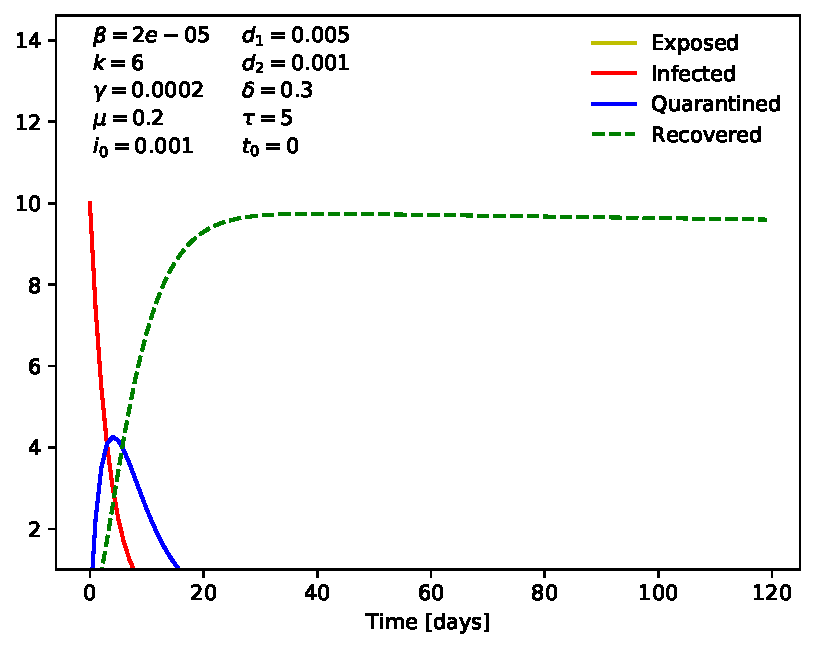
\includegraphics[width=0.4\textwidth]{imgs/ModelDescription/Summary_parameters_nominal.pdf}}
\subfloat[\label{fig:model_literature_modified}
]{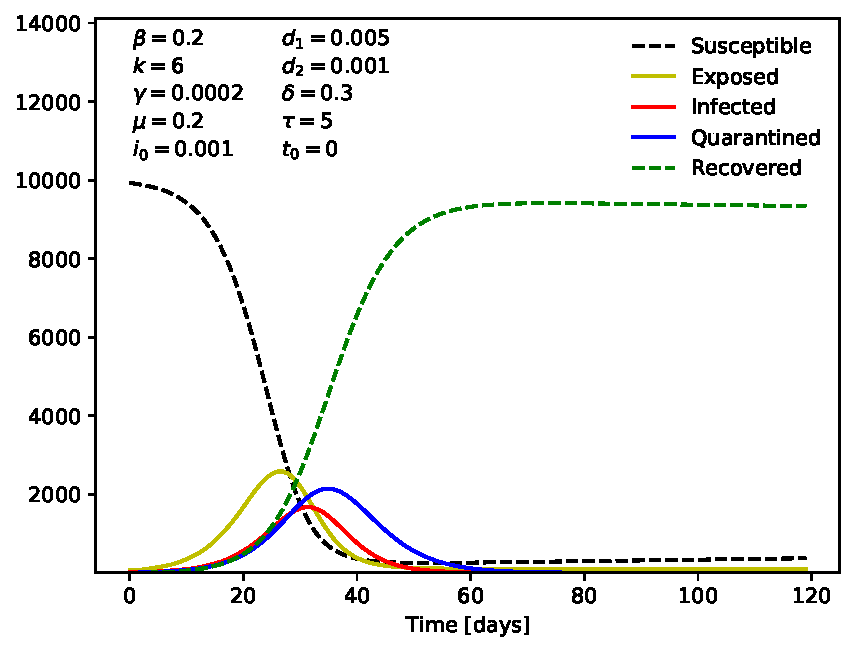
\includegraphics[width=0.42\textwidth]{imgs/ModelDescription/Summary_parameters_alternative.pdf}}
\caption{Numerical prediction of the model with different settings of the parameters. Parameters in Table~\ref{tab:literature_parameters} are used in (a), as well as in (b) but for $\beta=0.2$.}.
\end{figure}


\subsection{Impact of parameters on model predictions}
In this subsection the impact of the parameters on the model predictions is analysed. The most important parameters for the evolution of the infected population and the occurrence of the outbreak are $\beta$ and $\braket{k}$ parameters. The $\beta$ parameters is connected to the infection factor, so the probability of infecting a susceptible person in contact with and infected one. The $\braket{k}$ parameters indicate instead the number of connection for each individual, so measures the level of interaction of the small world. Since the two parameters always come together their effect is the same on the evolution and visible in Figure~\ref{fig:scan_i_vs_beta}, the larger those parameters are the steeper is the curve of the infected population, as expected from Equation~\ref{eqn:idot}.  A large impact on the outbreak evolution is also given by the fraction of quarantined infected population $\delta$, as shown in Figures~\ref{fig:scan_i_vs_delta} and \ref{fig:scan_q_vs_delta}. The outbreak is significantly contained in case a larger fraction of infected population is spotted and quarantined.

\begin{figure}[!ht]\centering
\subfloat[\label{fig:scan_i_vs_beta}]{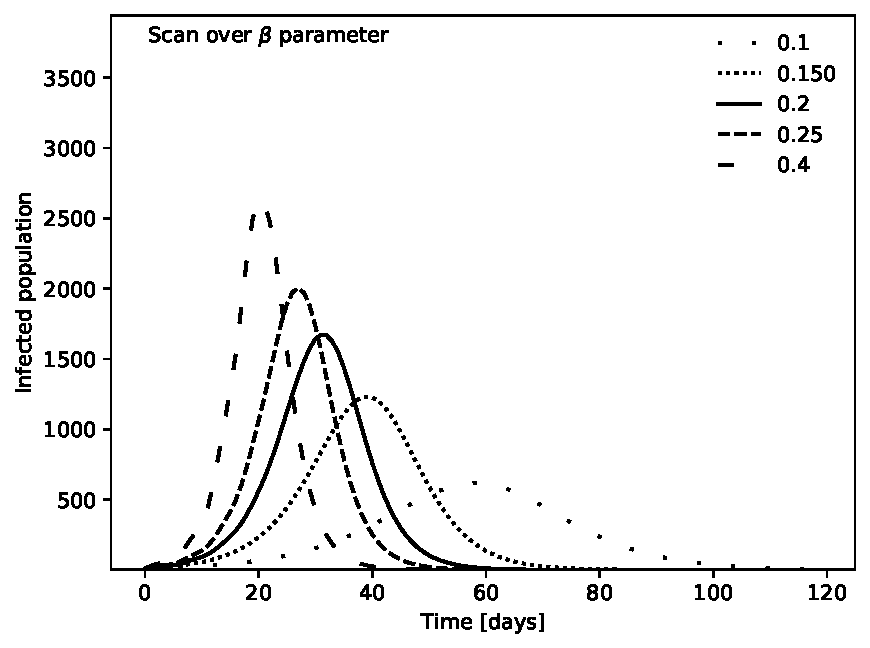
\includegraphics[width=0.32\textwidth]{imgs/ModelDescription/Scan_I_vs_beta_parameters_alternative.pdf}}
\subfloat[\label{fig:scan_i_vs_delta}]{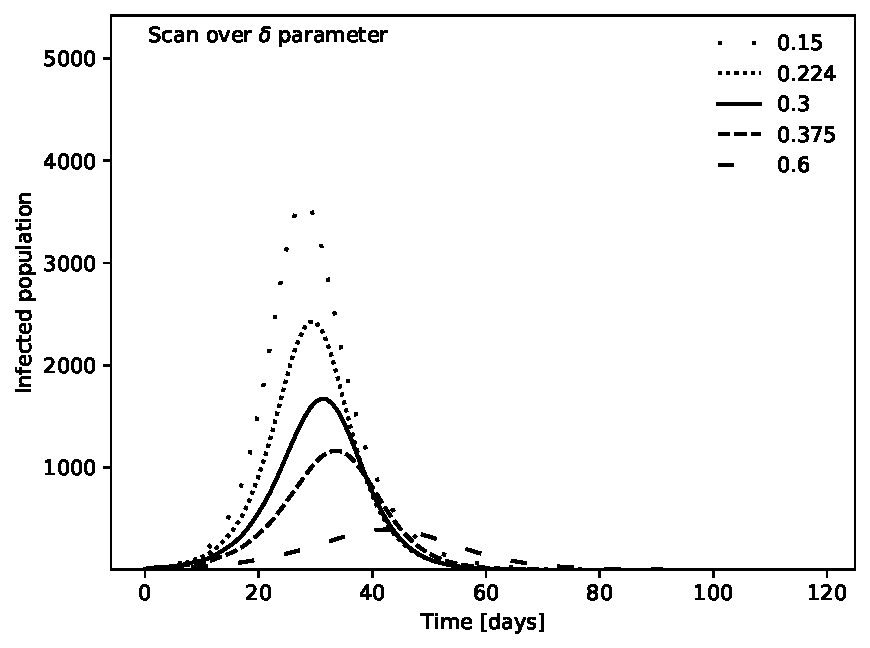
\includegraphics[width=0.32\textwidth]{imgs/ModelDescription/Scan_I_vs_delta_parameters_alternative.pdf}}
\subfloat[\label{fig:scan_q_vs_delta}]{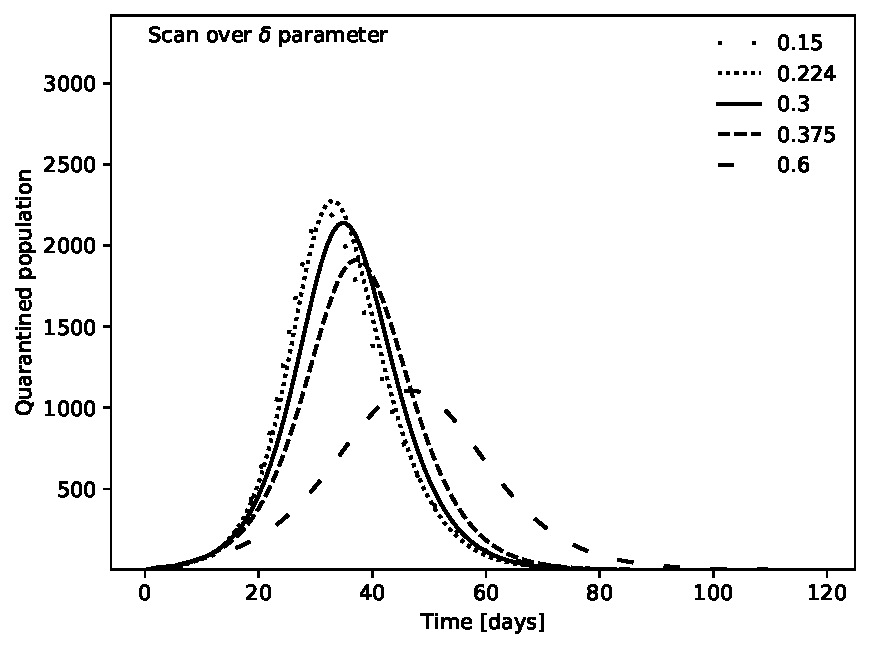
\includegraphics[width=0.32\textwidth]{imgs/ModelDescription/Scan_Q_vs_delta_parameters_alternative.pdf}}
\caption{Effect on the evolution of the infected population given by varying the $\beta$ parameter (a). Effect on infected (b) and quarantined (c) population given by varying the $\delta$ parameter.}.
\end{figure}

Other effects are given by $\gamma$, $\mu$ and $d_{1/2}$ parameters. Those control more the recovery curve. The $\gamma$ parameter is related to the probability of a recovered individual to not develop immunity: as shown in Figure~\ref{fig:scan_r_vs_gamma}, the recovered people has a decrease after the peak of the outbreak. The recovery curve is strongly affected by the $\mu$ parameter that regulates the recovery probability of the infected population: as shown in Figure~\ref{fig:scan_r_vs_mu}. The mortality $d_{1/2}$ instead increases the number of deaths, given by the difference of the recovered population and the initial $10000$ susceptible people, shown in Figure~\ref{fig:scan_r_vs_d1}.

\begin{figure}[!ht]\centering
\subfloat[\label{fig:scan_r_vs_gamma}]{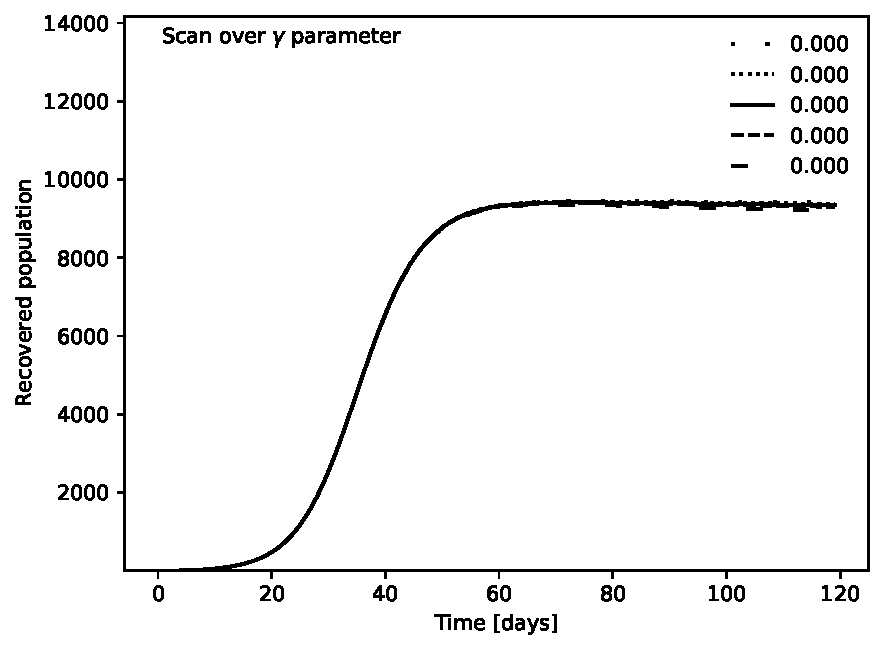
\includegraphics[width=0.32\textwidth]{imgs/ModelDescription/Scan_R_vs_gamma_parameters_alternative.pdf}}
\subfloat[\label{fig:scan_r_vs_mu}]{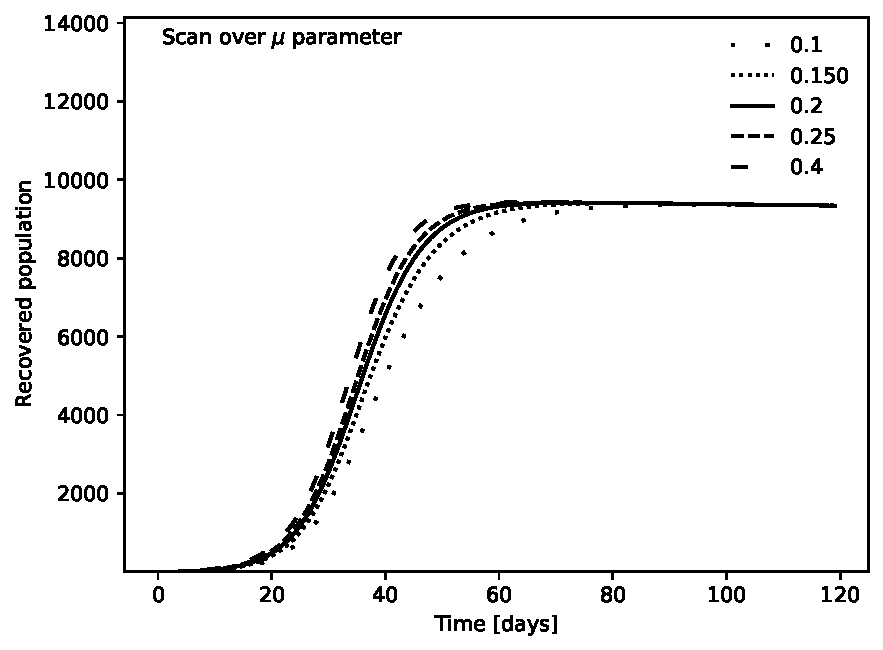
\includegraphics[width=0.32\textwidth]{imgs/ModelDescription/Scan_R_vs_mu_parameters_alternative.pdf}}
\subfloat[\label{fig:scan_r_vs_d1}]{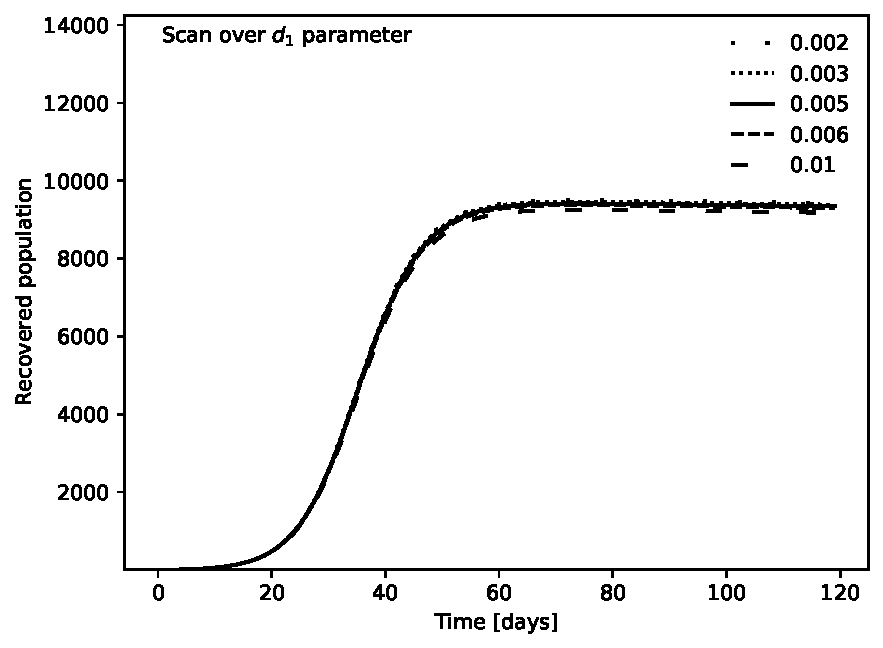
\includegraphics[width=0.32\textwidth]{imgs/ModelDescription/Scan_R_vs_d1_parameters_alternative.pdf}}
\caption{Effect on the evolution of the recovered population given by varying the $\gamma$ (a), $\mu$ (b) and $d_1$ (c) parameters.}.
\end{figure}

The only temporal parameter is the incubation time $\tau$: it also strongly affects the evolution of the oubreak, shown in Figure~\ref{fig:scan_i_vs_tau}. In case of long incubation time, the outbreak develops a  multiple peak structure, while in case of a short incubation time a clean gaussian peak is recognised.

\begin{figure}[!ht]\centering
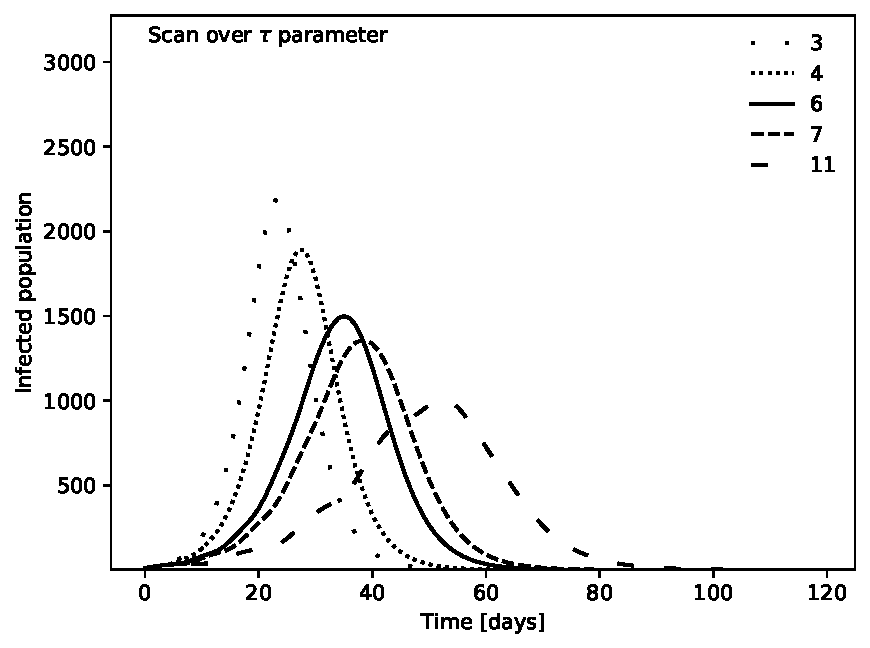
\includegraphics[width=0.4\textwidth]{imgs/ModelDescription/Scan_I_vs_tau_parameters_alternative.pdf}
\caption{Effect on the evolution of the infected population given by varying the $\tau$ parameter.}
\label{fig:scan_i_vs_tau}
\end{figure}


\section{Dataset}

The dataset used to test the predictability of the developed model are about the COVID-19 oubreak in Italy. This dataset is used because the quarantine procedure has been implemented quite at the beginning of the outbreak, as in the model. Moreover Italy is a high-density country, especially in the Lombardy area, so that the small-world approximation may be feasible to describe the oubreak. Data are extracted from the web-site of \emph{Il Sole 24 Ore} \cite{Lab24}, the main economical italian newspaper, that has been one of the first sources of data divided by regions. Data in Italy and Lombardy are shown in Figures~\ref{fig:data_italy} and \ref{fig:data_lombardy}.\\

\begin{figure}[!ht]\centering
\subfloat[\label{fig:data_italy}]{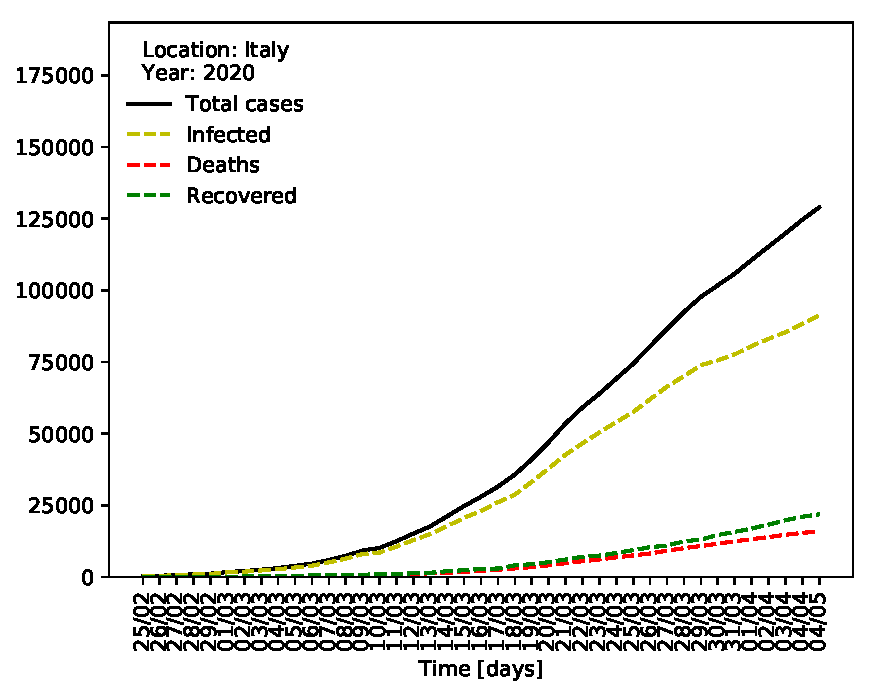
\includegraphics[width=0.4\textwidth]{imgs/Dataset/Data_Italy.pdf}}
\subfloat[\label{fig:data_lombardy}]{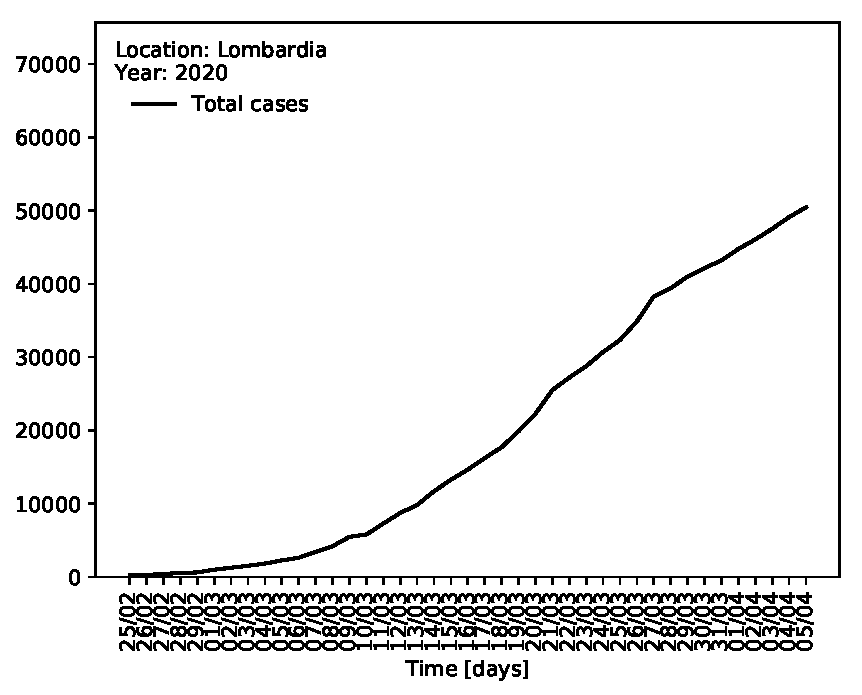
\includegraphics[width=0.4\textwidth]{imgs/Dataset/Data_Lombardia.pdf}}

\caption{Dataset collected in Italy (a) and Lombardy (b).}.
\end{figure}

A focus on Lombardy dataset is given, since it is by far the most affected region in Italy, completely driving the numbers of the outbreak in the whole country, and it is smaller, high-populated, very dynamic and connected area, where small-world approximation may work better.
\section{Application to the COVID-19 outbreak}
\label{sec:covid}

The mathematical model described in Section~\ref{sec:model} is checked against data of the oubreak in Lombardy in  Figure~\ref{fig:data_lombardy}. \\

The dataset indicates only the total cases, corresponding to positive tested population, deaths and recovered people. In the model, this quantity is estimated by the sum of quarantined $Q$, deaths $D$ and recovered $R$ categories. The infected and exposed population is here not considered due to the testing campaign adopted in Lombardy. Only people with a chance of having contracted the virus (medical staff, people close to positive cases) and infected people developing heavy symptoms to need hospitalisation. Since exposed and infected categories contain individuals with the virus but with at most mild symptoms, they are not tested and are not included in the numbers of  positive  cases. The quarantined category contain people getting hospitalised and therefore being immediately quarantined by the medical structure. \\

Since the plateau of the total cases is not reached in data, the most important parameters to tune to agree with the collected data are $\beta$, $\braket{k}$, $\delta$ and $\tau$ parameters. On top of the parameters described in Section~\ref{sec:model}, an additional parameter $t_0$ has been added to shift the distribution in time. The  prediction that matches at most with data, after tuning the model parameters, is shown in Figure~\ref{fig:data_vs_model_first_lombardy}. Parameters modifying the trailing edge of the infection is set to approximate values of the outbreak. Mortality is set to $2\%$, reinfection probability to $10^{-5}$ since yet no cases have been observed. Population is set to $10^7$, corresponding to Lombardy population.\\

\begin{figure}
\centering
  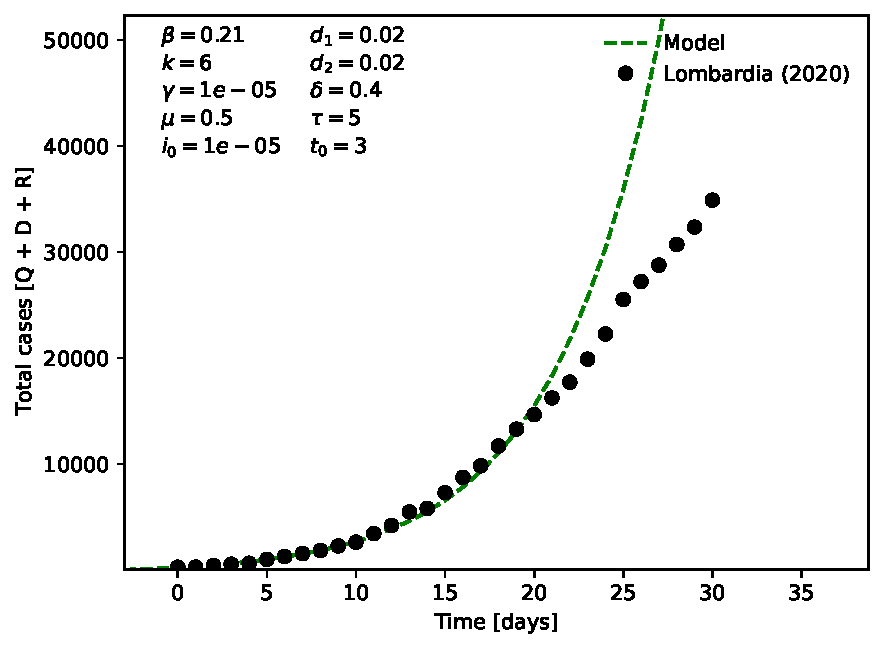
\includegraphics[width=0.4\textwidth]{imgs/Covid/DataVsModel_parameters_Lombardia_less_impacting.pdf}
  \caption{Best match of parameters to make the model described in Section~\ref{sec:model} fit with data il Lombardy.}
  \label{fig:data_vs_model_first_lombardy}
\end{figure}

As shown in Figure~\ref{fig:data_vs_model_first_lombardy} the model predicts an exponential growth until the peak, that is not what is measured, since different slopes of curve are present in data. The hypothesis is that the parameters of the model changes in time due to the several restrictions applied to social activity to contain the virus spreading  (non-essential activities closed, cancellations of events, etc.). These regulations cause a decrease of the total cases slope, impossible to predict with the mathematical implant of Section~\ref{sec:model}. \\

Two main measures to contain the virus have been introduced since March 1st, when the outbreak started to significantly spread. The first strong limitations have been introduced on March 9th \cite{DPCM-0903} and 11th \cite{DPCM-1103}, the so-called \emph{\#iorestoacasa} laws, forcing non-essential activities to close and encouraging home-quarantine. More stringent laws, prohibiting any movement outside the city of residence and forcing the lock-down except for emergencies, have been released on March 20th \cite{DPCM-2003} and 22th \cite{DPCM-2203}. This regulations are still valid at the time of writing (April 15th). Indeed, around those dates, the slopes of the total cases curves change, confirming that these procedures have been important to contain the spreading of the virus. The mathematical model described in Section~\ref{sec:model} is then modified to reflects these changes and to model better the data behaviour.

\subsection{Adapting the model to real-world scenario}
\label{ssec:impr_model}


To adapt the model to the real world scenario, few improvements have been implemented:
\begin{itemize}
\item Inclusion of a recovery rate for the infected category evolution.
\item Fluctuation of $\delta$ parameter: this reflects the fluctuation of the number of tests performed per day.
\item Scheduling of $\braket{k}$ parameter: this reflects the social-distancing measures.
\end{itemize}

A scheduling of the $\delta$ parameter is not introduced. This implies that the fraction of the infected people getting tested is almost constant over time. This assumption is reasonable since the testing strategy has been kept consistent over time. Indeed, the mortality rate, normalised by the number of tests, is quite flat.\\

The original model does not include a recovery rate for the infected category. Therefore an infected person is only expected to develop symptoms and get quarantined. A person heals only if quarantined before. This is not the real case, the infected people are identified as non-symptomatic contagious infected individuals, and they can recover from the virus without being hospitalised, tested and quarantined. Therefore the variation $\dot{i}$ is modified as follows:
\begin{equation}
\dot{i} (t)= \beta\braket{k}s(t-\tau)i(t-\tau) - d_1i(t) - \delta {i(t)} - \mu{i(t)}
\end{equation}
This part of recovered people are not counted in the recovered category.\\

Corrections of the $\delta$ parameter over time are derived to account for the non-constant rate of performed test and shown in Figure~\ref{fig:tests_vs_time}. A functional model has been fitted to the data points (taken from reference \cite{Lab24}) and the corrections are computed as ratio of the observed points with respect to the function. The function is consistent with the choice of a constant $\delta$ since it approximately describe the data trend in Figure~\ref{fig:data_lombardy}.\\

\begin{figure}
\centering
  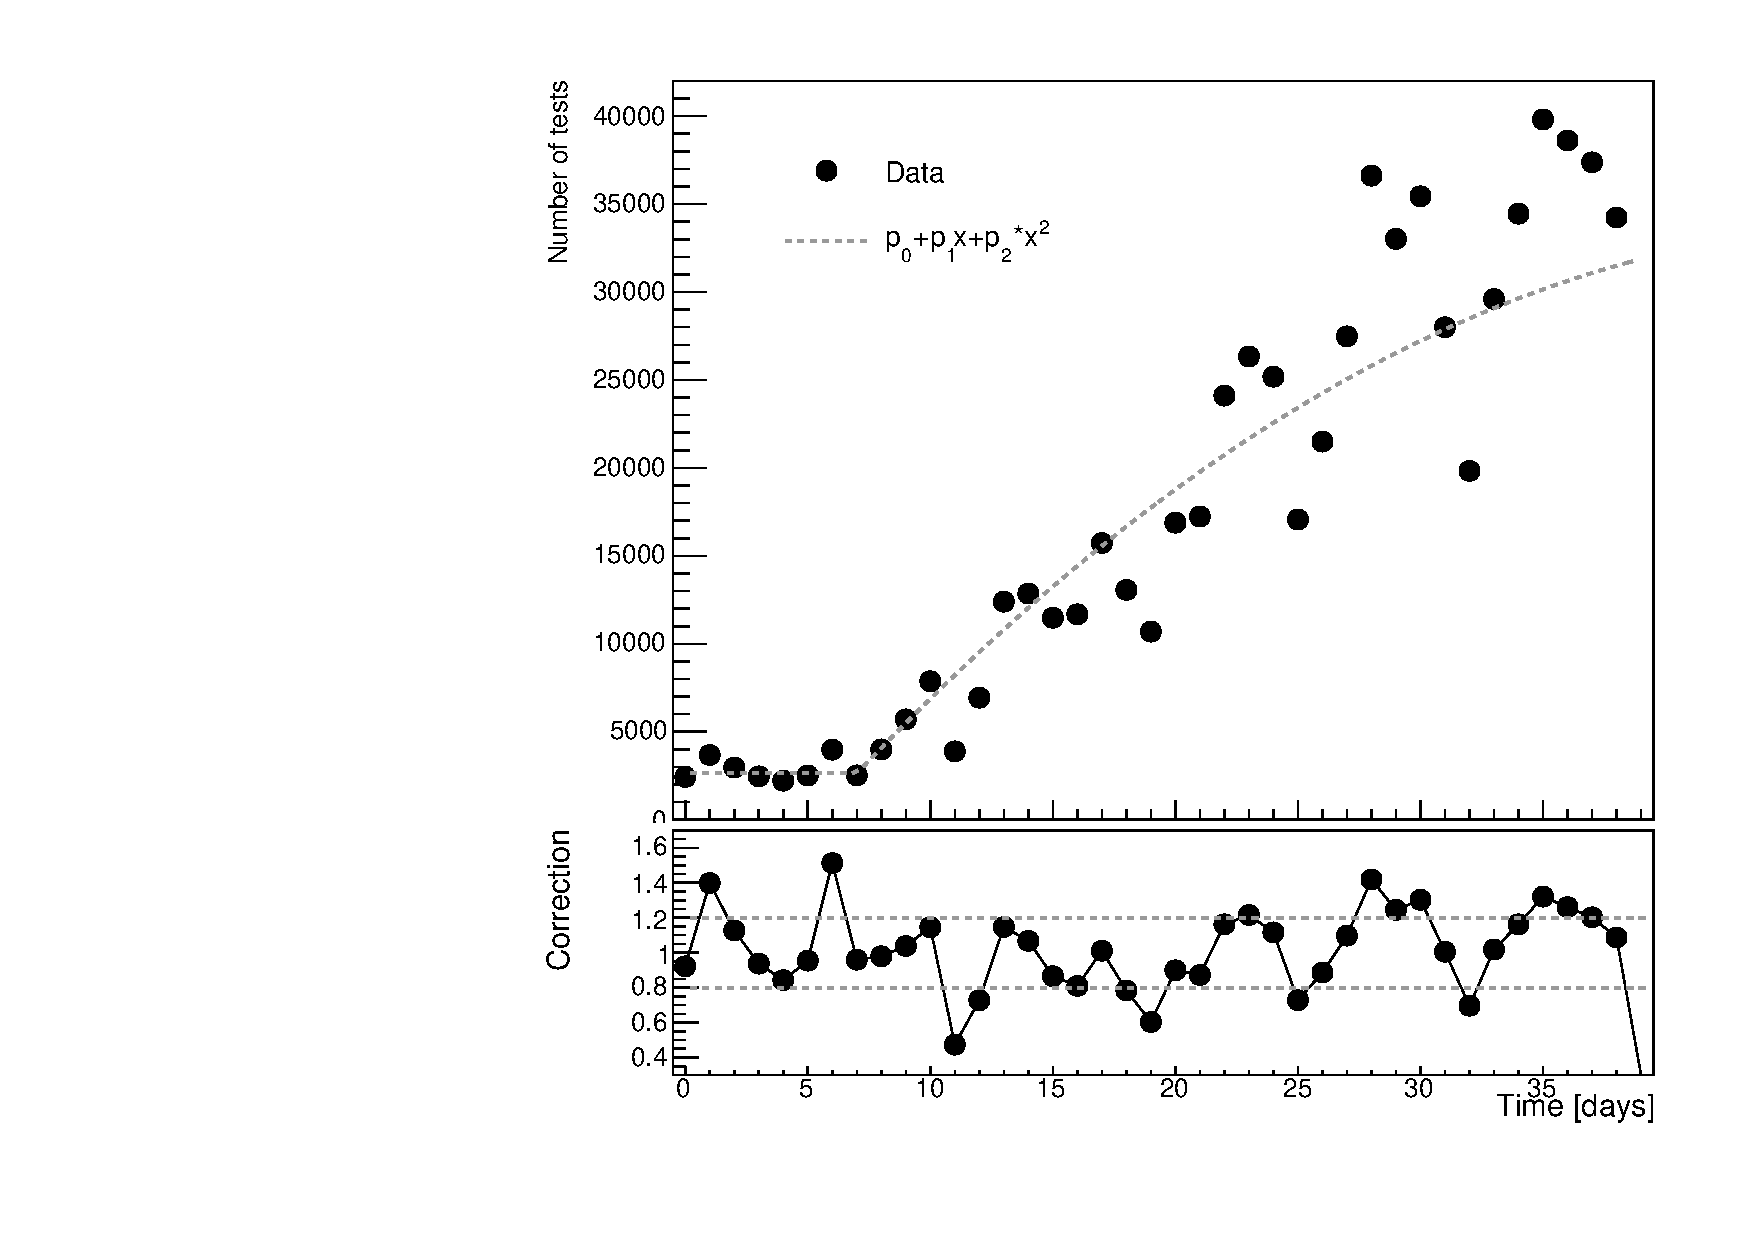
\includegraphics[width=0.4\textwidth]{imgs/Covid/TamponsCorrections.pdf}
  \caption{Numbers of performed tests over time in Italy. A constant plus a third degree polynominal is fitted and corrections (plot below) are extracted as a difference of the measured points to the functional model.}
  \label{fig:tests_vs_time}
\end{figure}

This correction is introduced to describe the non-smooth behaviour of the curve. However, since this data are available national-wise, the numbers for Lombardy may differ. This possible discrepancy is accounted in the fit, described in Section~\ref{ssec:plf}. \\

The $\braket{k}$ scheduling represents the introduction of social-distancing, varying from a freely-communicating system (where  $\braket{k}$ is set to the initial value) to the lock-down situation in which an infected person interact only with few susceptible individuals (family).\\

\begin{figure}
\centering
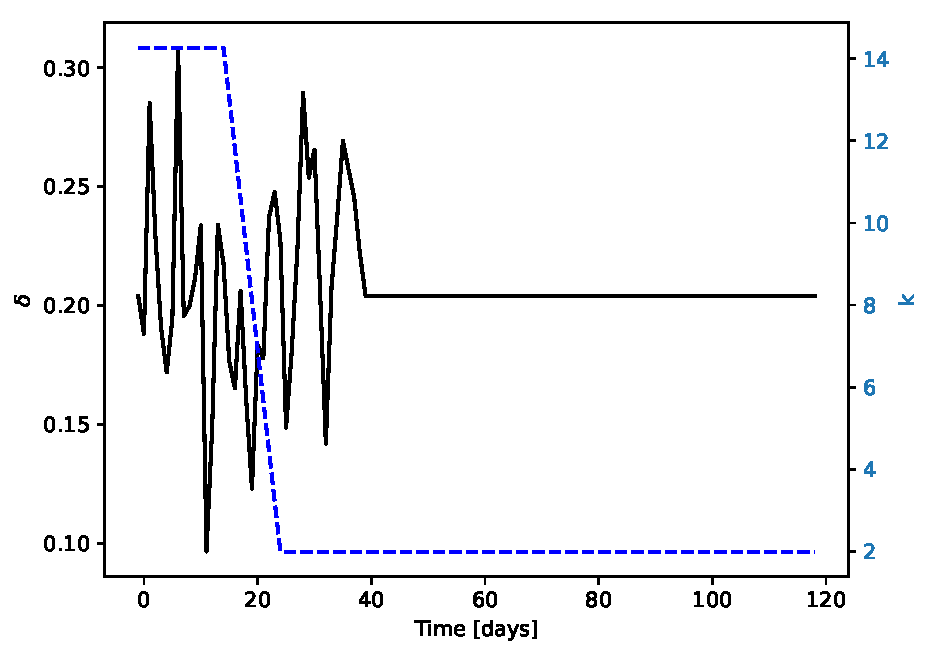
\includegraphics[width=0.4\textwidth]{imgs/Covid/Scheduling_regular.pdf} 
  \caption{Variations of $\delta$ and $\braket{k}$ parameters over time. The reference values of the parameters are set the same as in Figure~\ref{fig:data_vs_model_first_lombardy}.}
  \label{fig:scheduling}
\end{figure}

The values of $\delta$ and $\braket{k}$ parameters over time is shown in Figure~\ref{fig:scheduling}. A new set parameters is tuned to approximately match data shape. This new tuned prediction is shown in Figure~\ref{fig:model_vs_time}, while the comparison with data is presented in Figure~\ref{fig:model_vs_data}.\\

\begin{figure}
\centering
\subfloat[\label{fig:model_vs_time}]{ 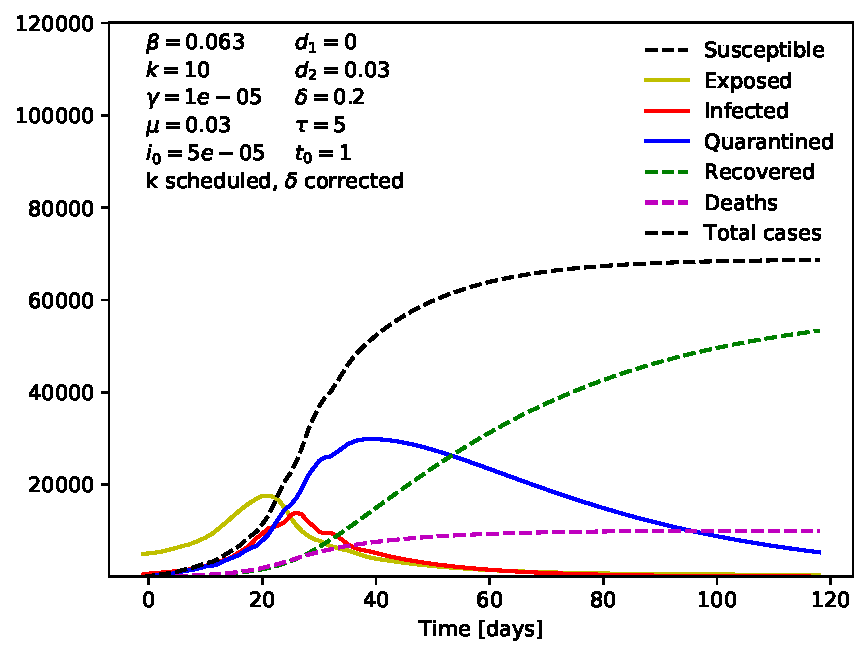
\includegraphics[width=0.4\textwidth]{imgs/Covid/Summary_parameters_Lombardia_scheduling_corrected_definitive_v2.pdf} }
\subfloat[\label{fig:model_vs_data}]{ 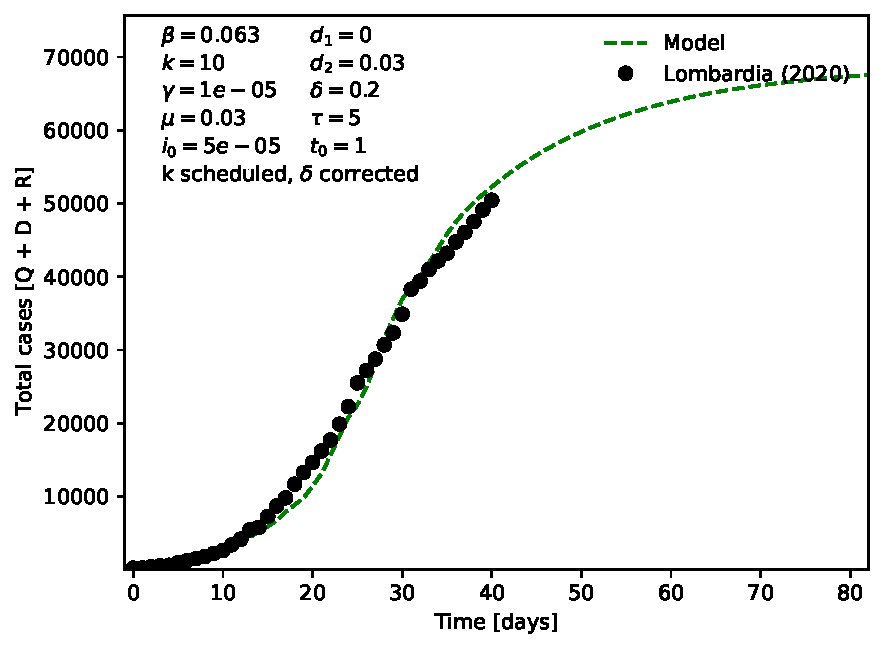
\includegraphics[width=0.4\textwidth]{imgs/Covid/DataVsModel_parameters_Lombardia_scheduling_corrected_definitive_v2.pdf} }
  \caption{Prediction of the improved model for the population classes with the correction with a new set of tuned parameters (a). Comparison of the model in (a) with the data collected in Lombardy (b).}
  
\end{figure}



\subsection{Profile likelihood fit to data}
\label{ssec:plf}

The model parameters are measured with a Profile Likelihood fit. The fit is performed using \textsc{ROOT} framework \cite{ROOT}, in particular with the \emph{HistFactory} framework to create statistical models \cite{HistFactory}.\\

The observable used in the fit is the daily number of total cases (deaths, quarantined and recovered) to use uncorrelated quantities for each bin of the fitted distribution. The distribuition is rebinned to increase statistics per bin. The Parameter of Interest (PoI) is a global normalisation factor of the distribution, introduced as a free floating parameter. This corresponds to a variation of the initial condition, $i_0$, that is not included in the set of parameters to fit. The profile likelihood fit adjusts the model parameters to maximise the likelihood of the data given the assumed model \cite{HistFactory}.\\
  
Since no functional model is available, templates of the total cases distribution for different choices of the model parameters are generated and used in the fit. For each parameter of the model, two templates of the distribution are generated, corresponding of increasing and decreasing of a $10\%$ the parameter value. A nuisance parameter (NP)of the model, with Normal Gaussian prior, is associated to each model parameter used in the fit. The variation of each template from the nominal predictions given by the variation of a single parameter is associated to the variation of the associated NP, whose $\pm1$ standard variation correspond to the two differences of the templeates in input. For middle values of the NP, an interpolation is used bin-by-bin, to get the corresponding effect of the parameter on the distribution. An example of the effect of the variation of a model parameter is shown in Figure~\ref{fig:alpha_beta}. To improve the fit stability the effect of the NPs are symmetrised against the nominal prediction. In case both variations are on one side, as in Figure~\ref{fig:syst_np}b, the variation is one-sided symmetrised.\\

\begin{figure}
\centering
\subfloat[\label{fig:alpha_beta}]{ 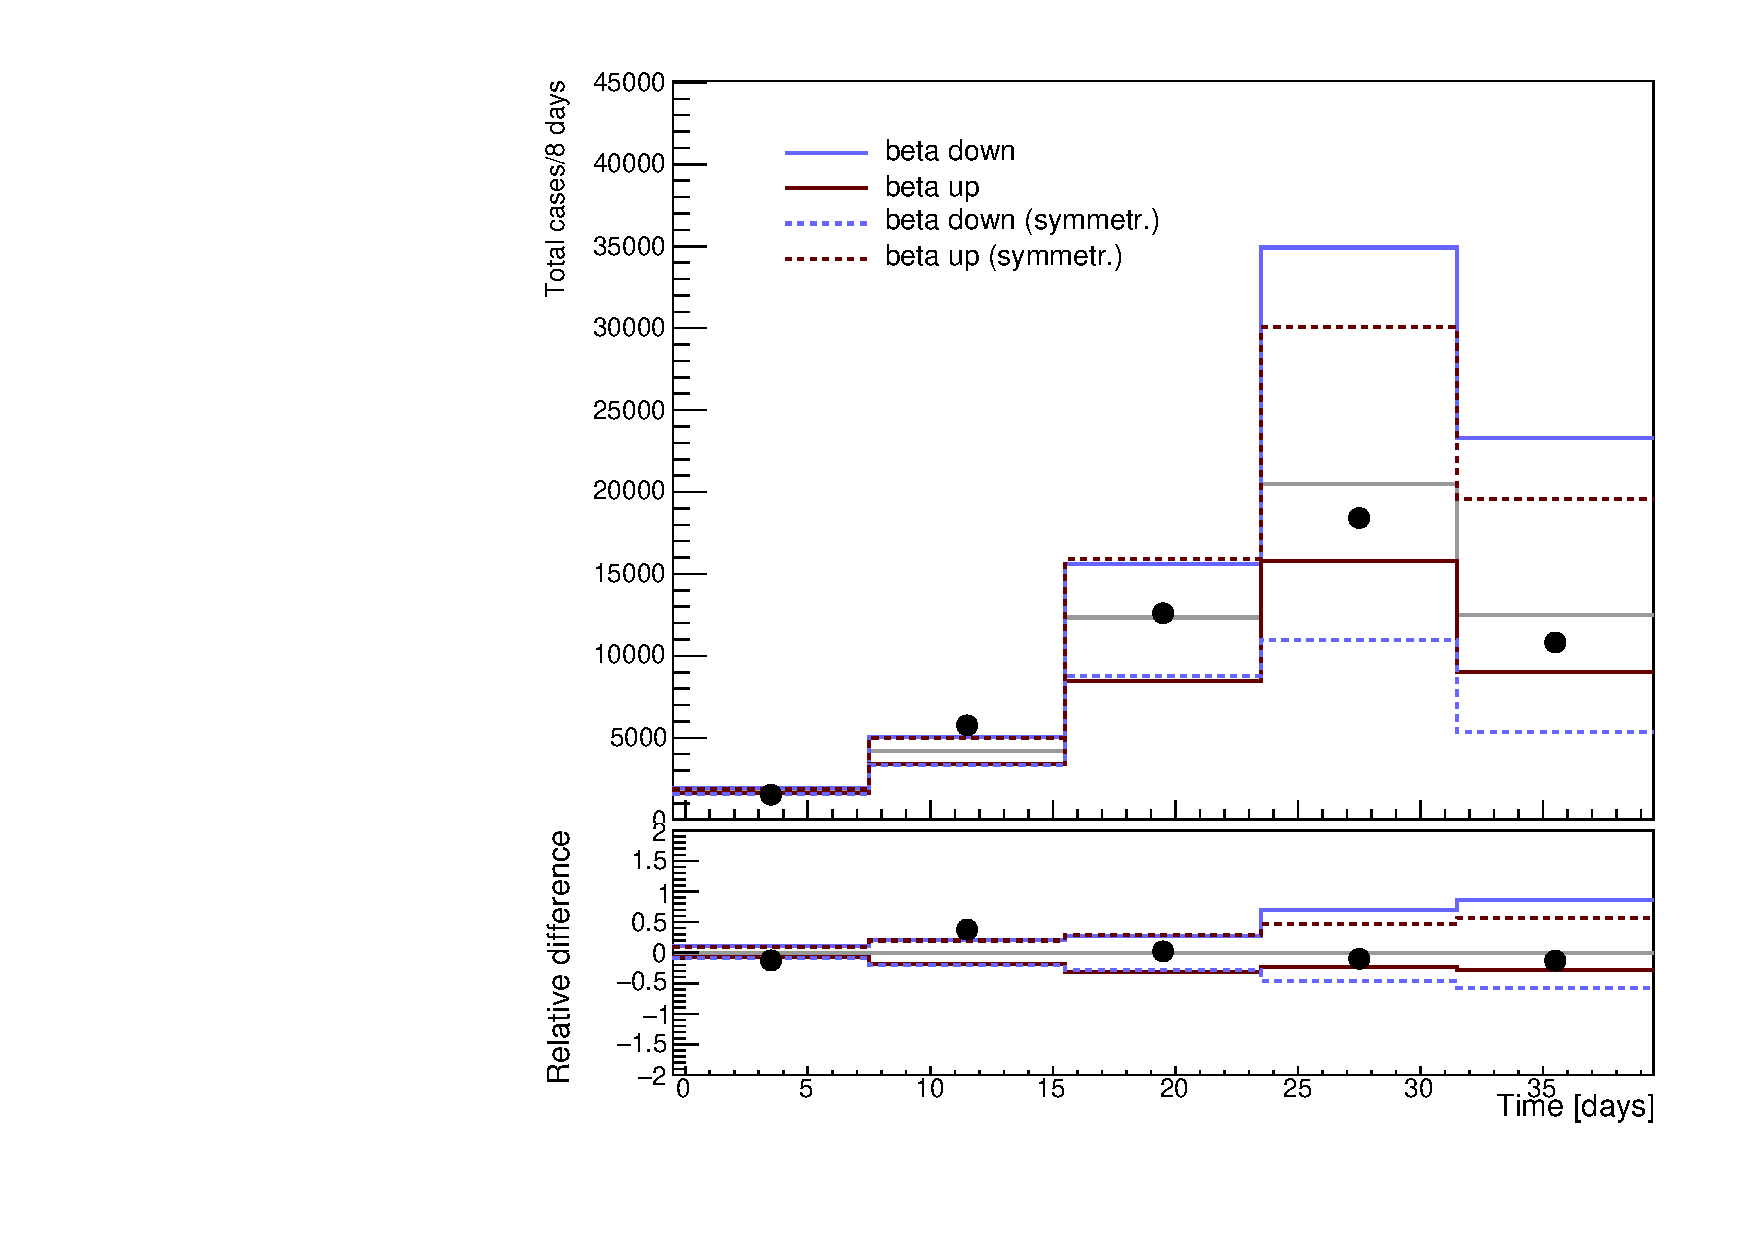
\includegraphics[width=0.4\textwidth]{imgs/Covid/Syst_beta.pdf} }
\subfloat[\label{fig:alpha_mu}]{ 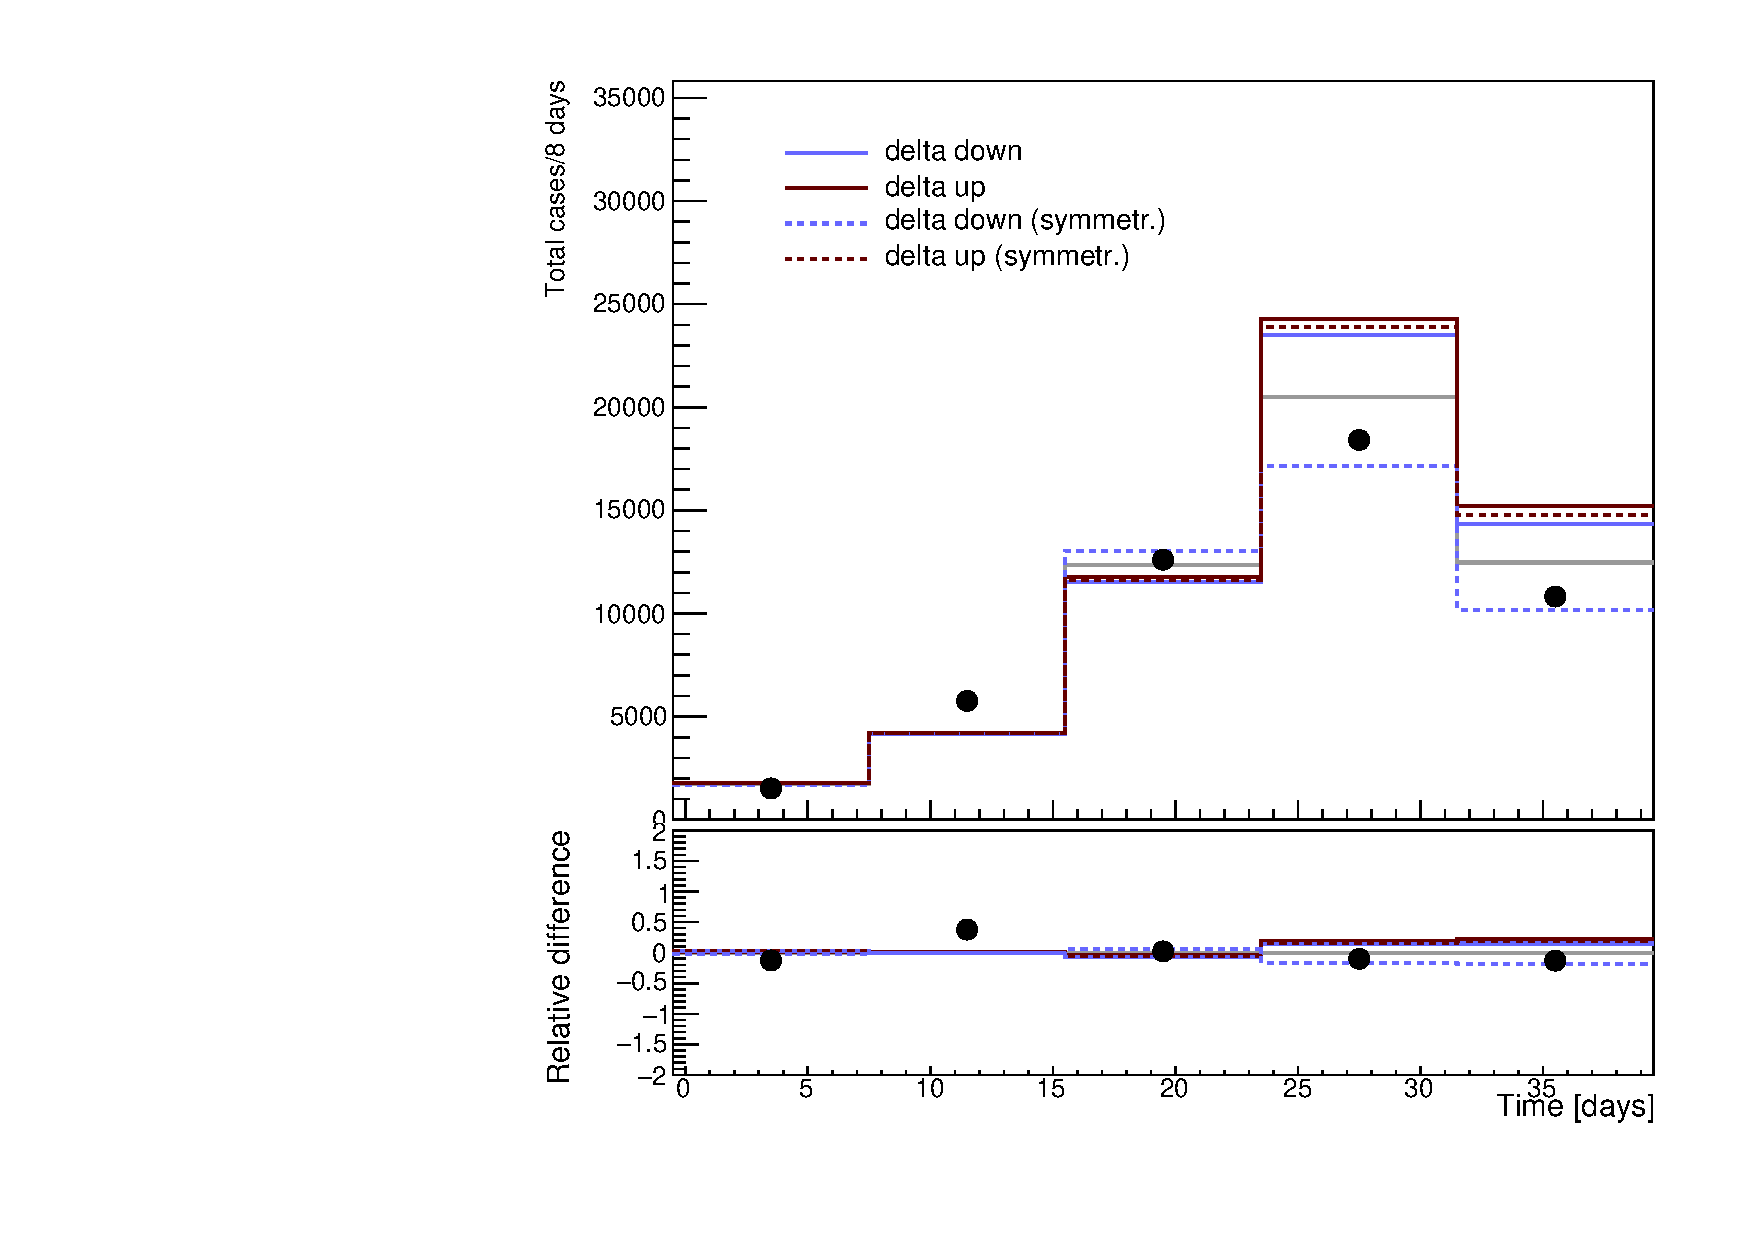
\includegraphics[width=0.4\textwidth]{imgs/Covid/Syst_delta.pdf} }
  \caption{Two examples of NPs included in the fit: variation of $\beta$ (a) and $\delta$ (b) parameters. In the $\delta$ parameter case, a one direction effect of the parameter is expected. A higher value of $\delta$ increases the number of quarantined people per day.  A lower value of $\delta$ instead makes the spreading faster, increasing the number of infected and then of quarantined people as well. In both plots the effect of the symmetrised variation is shown.}
  \label{fig:syst_np}
\end{figure}

To give enough degrees of freedom to the fit, additional NPs are used to take into account uncertainties on the $\delta$ correction described in Section~\ref{ssec:impr_model}. From Figure~\ref{fig:tests_vs_time}, a variance of $20\%$ is estimated, and a NP for each bin is added, assuming that the variations are uncorrelated bin-by-bin. The example for the two highest bins are shown in Figure~\ref{fig:syst_np_corrbin}.\\

\begin{figure}
\centering
\subfloat[]{ 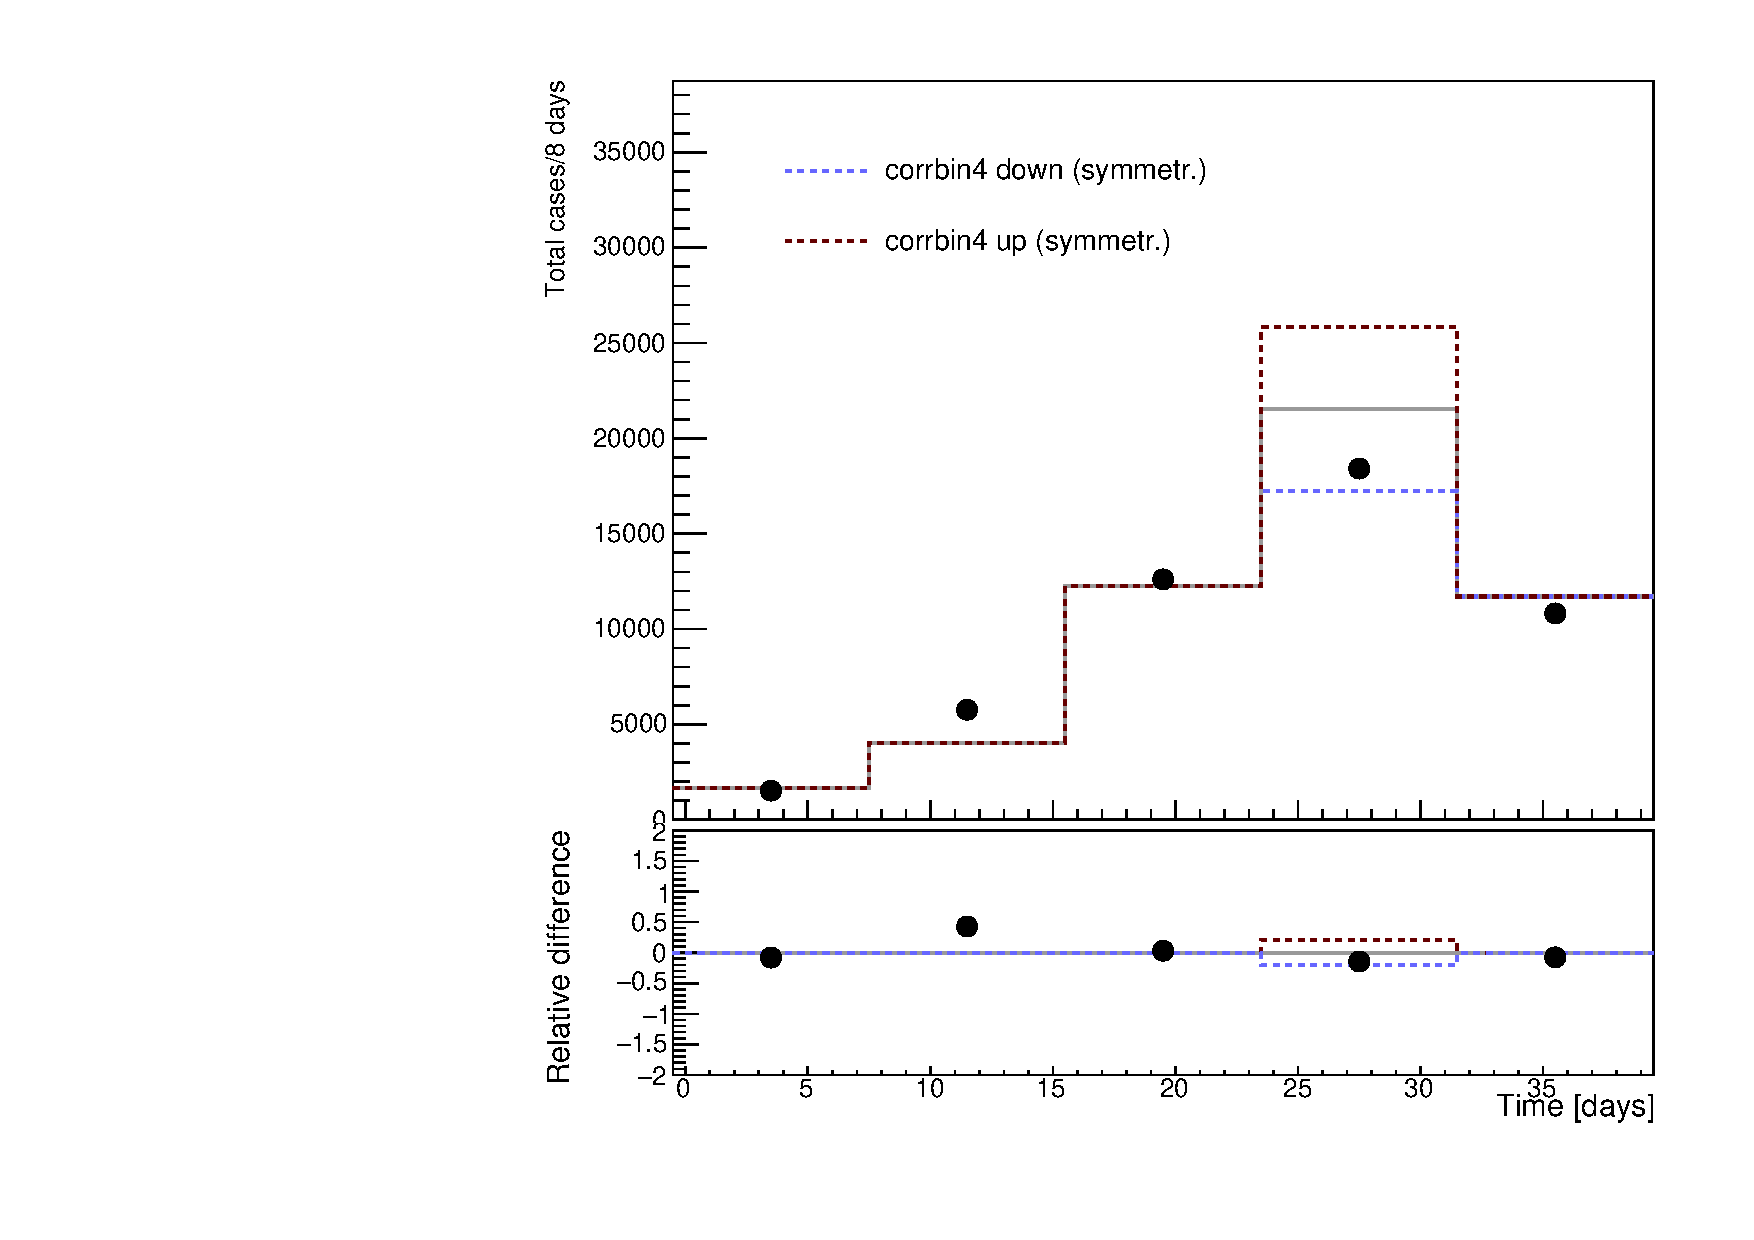
\includegraphics[width=0.4\textwidth]{imgs/Covid/Syst_corrbin4.pdf} }
\subfloat[]{ 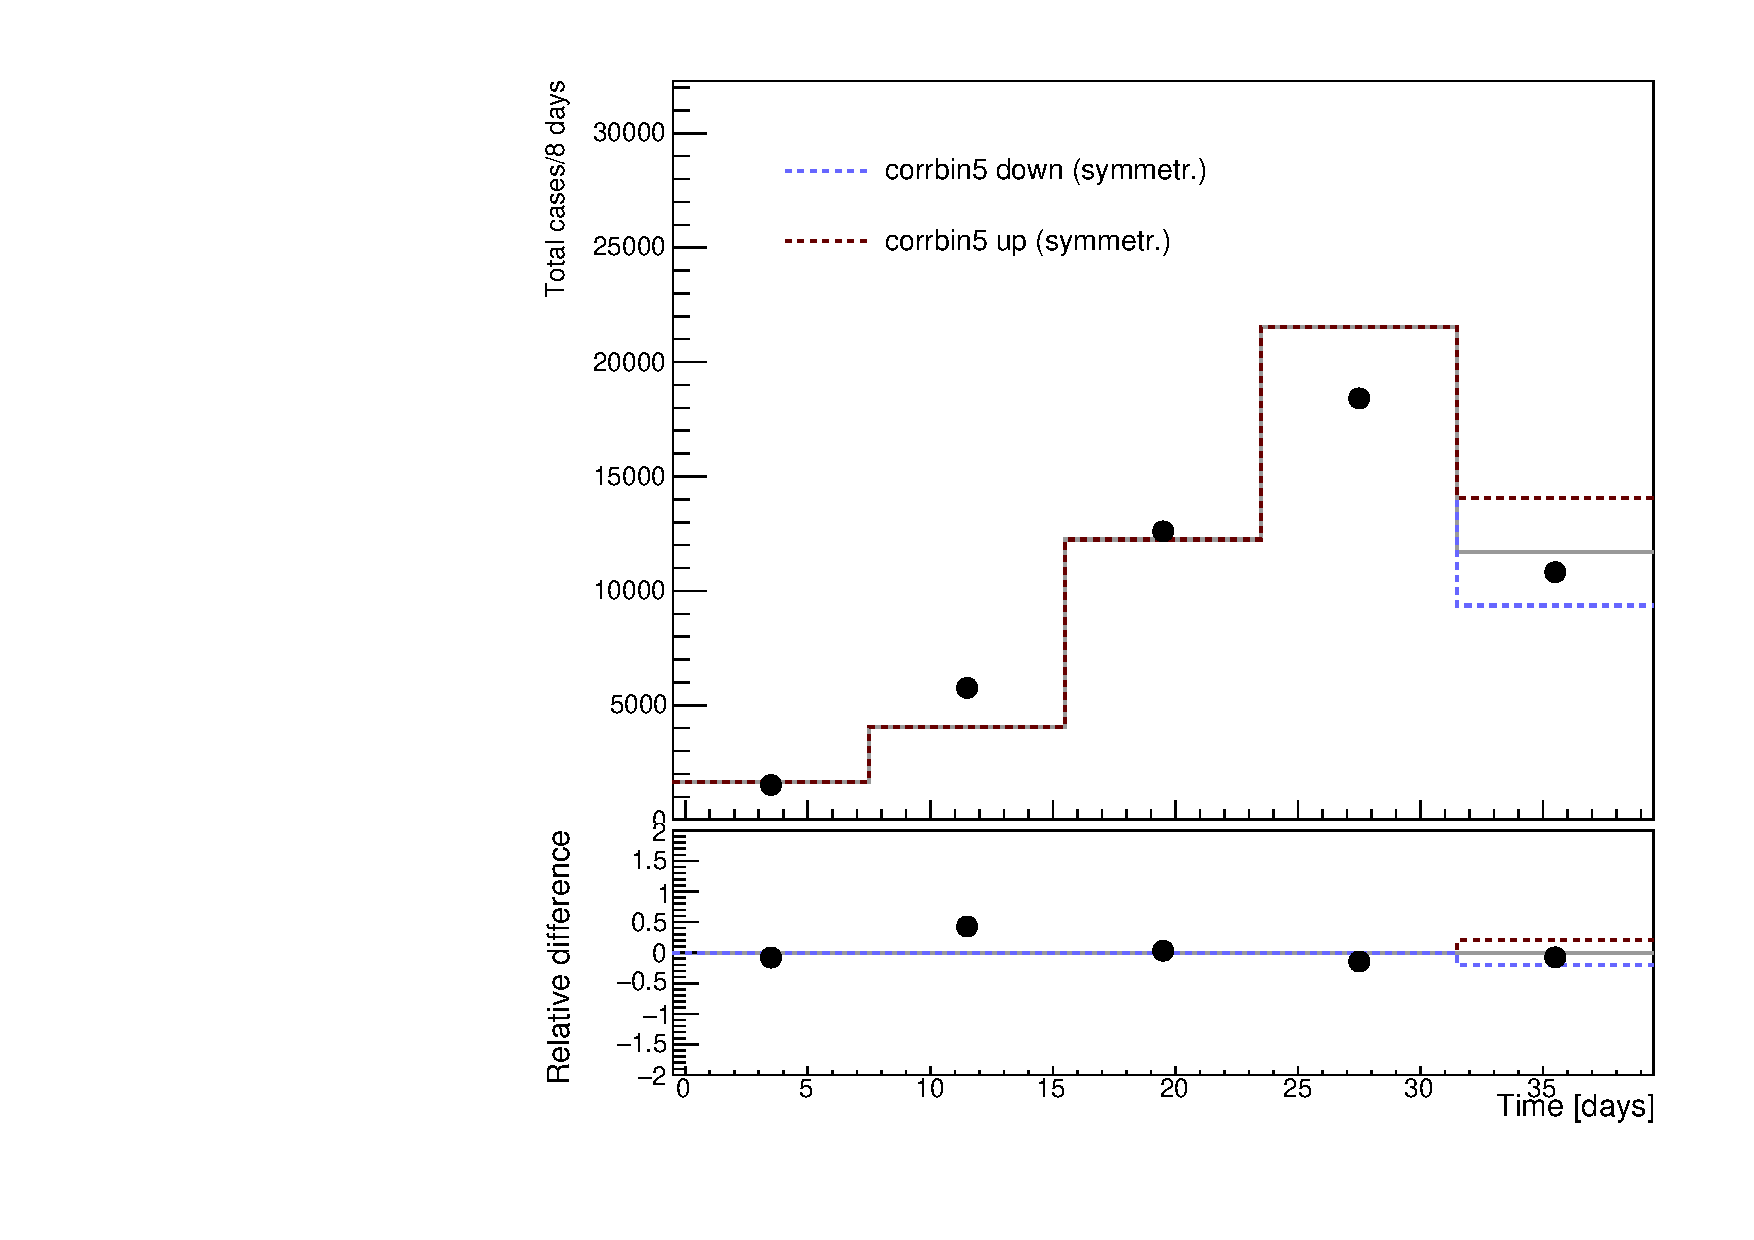
\includegraphics[width=0.4\textwidth]{imgs/Covid/Syst_corrbin5.pdf} }
  \caption{Variations associated to the test-based $\delta$ parameter corrections on the most significant bins in terms of the shape of the outbreak spreading.}
  \label{fig:syst_np_corrbin}
\end{figure}

The pre-fit prediction is shown in Figure~\ref{fig:prefit}, showing a good agreement of the data with the model withing the (large) uncertainties. The summary of the fitted model parameters and their correlations are shown in Figure~\ref{fig:nps}. Figure~\ref{fig:nps}a shows the pre-fit NPs value, equal to zero, following a Normal Gaussian distribution. The points indicate the post-fit values and associated uncertainties. The uncertainties on the parameters are constrained, meaning that the assumed systematics model is conservative and the NPs are measured with a higher precision than the assumptions. This is acceptable, since the used $10\%$ uncertainty on the parameters is set arbitrarily, choosing the smallest uncertainty range for all the parameters that cover the discrepancies of the model with data. Large pulls, over one standard deviations are observed in just two NPs, corresponding to the correcions on the bin contents. This is acceptable as well since the  uncertainty on those two parameters are estimated assuming the Gaussian fluctuations on the fitted model in Figure~\ref{fig:tests_vs_time}. In case the Lombardy tests are way different from the coutry-wise data in some periods, this assumption is not valid and pulls may appear. The parameter of interest, denoted as \emph{SF}, is expected to be unitary and still fitted consistently to the expectaion within one standard deviation. Correlations between parameters are understood: the scale factor, $\beta$, $\tau$ and the bin corrections are the most correlated, since they are the most important parameter to change the distribution shape in the fit range. The correlations are coherent with the expectations since they tend to counter-balance the different effects among themselves to agree with the data distribution. \\

\begin{figure}
\centering
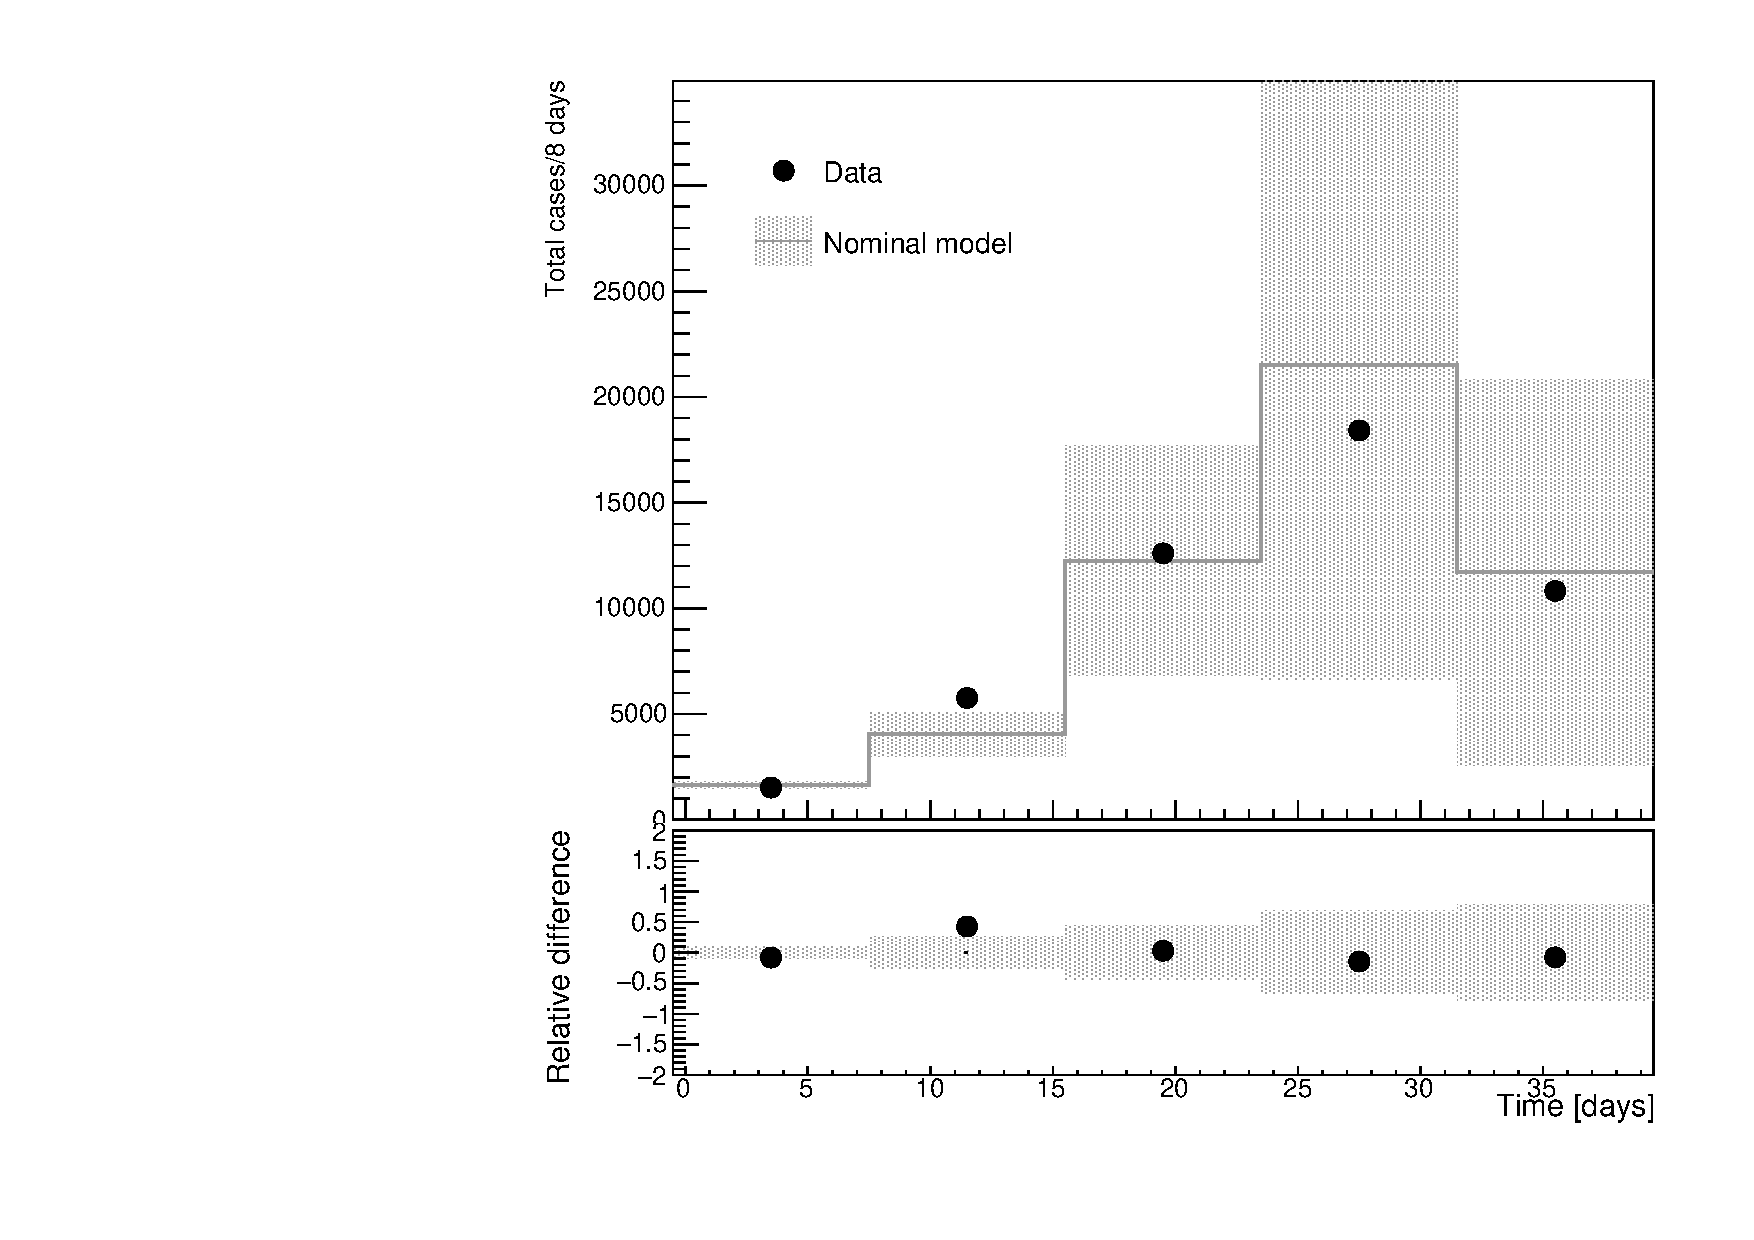
\includegraphics[width=0.4\textwidth]{imgs/Covid/ModelPrefit.pdf} 
  \caption{Pre-fit prediction of the model with the corrections described in Figure~\ref{ssec:impr_model} and the parameters in Figure~\ref{fig:model_vs_time}. The total uncertainty is given by summing all the sources of uncertainties described in Section~\ref{ssec:plf}}
  \label{fig:prefit}
\end{figure}

\begin{figure}
\centering
\subfloat[]{ 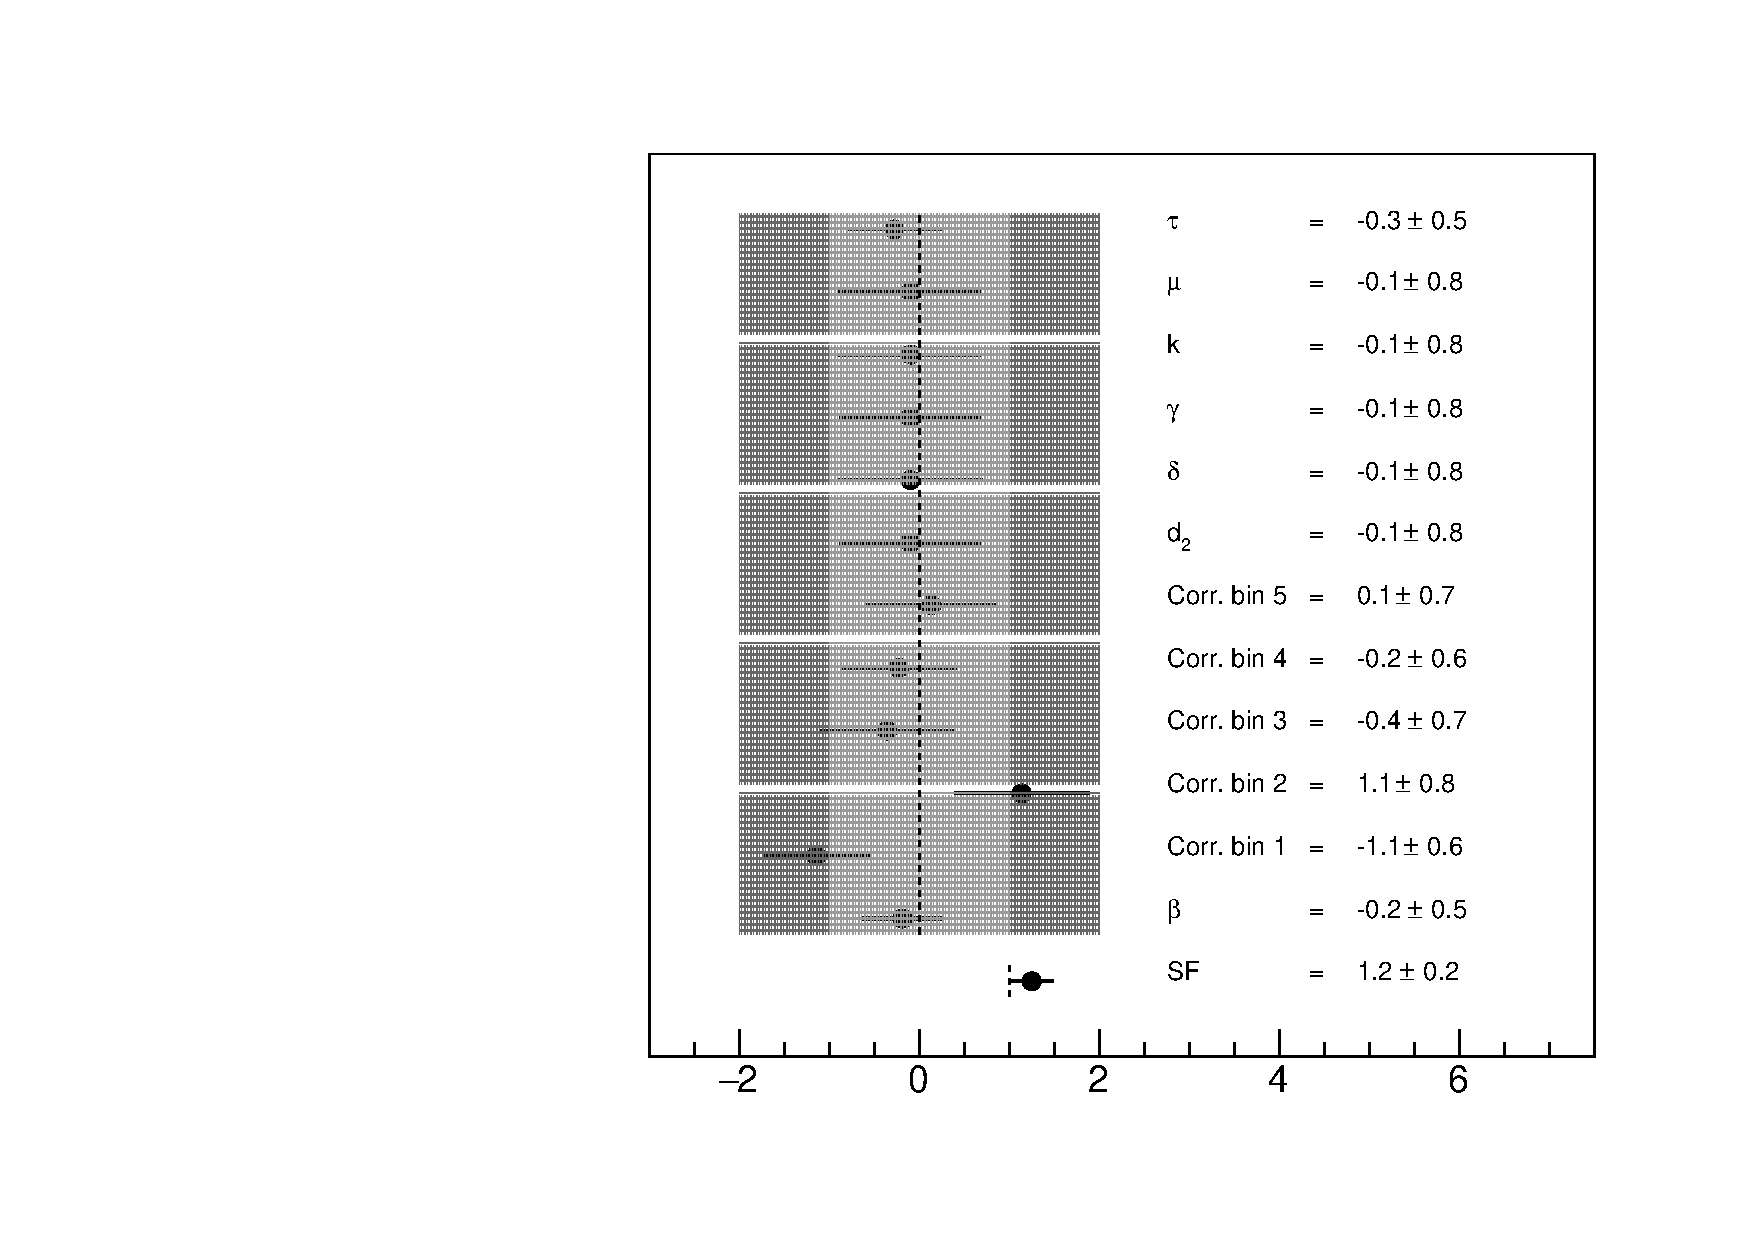
\includegraphics[width=0.45\textwidth]{imgs/Covid/PoI.pdf} }
\subfloat[]{ 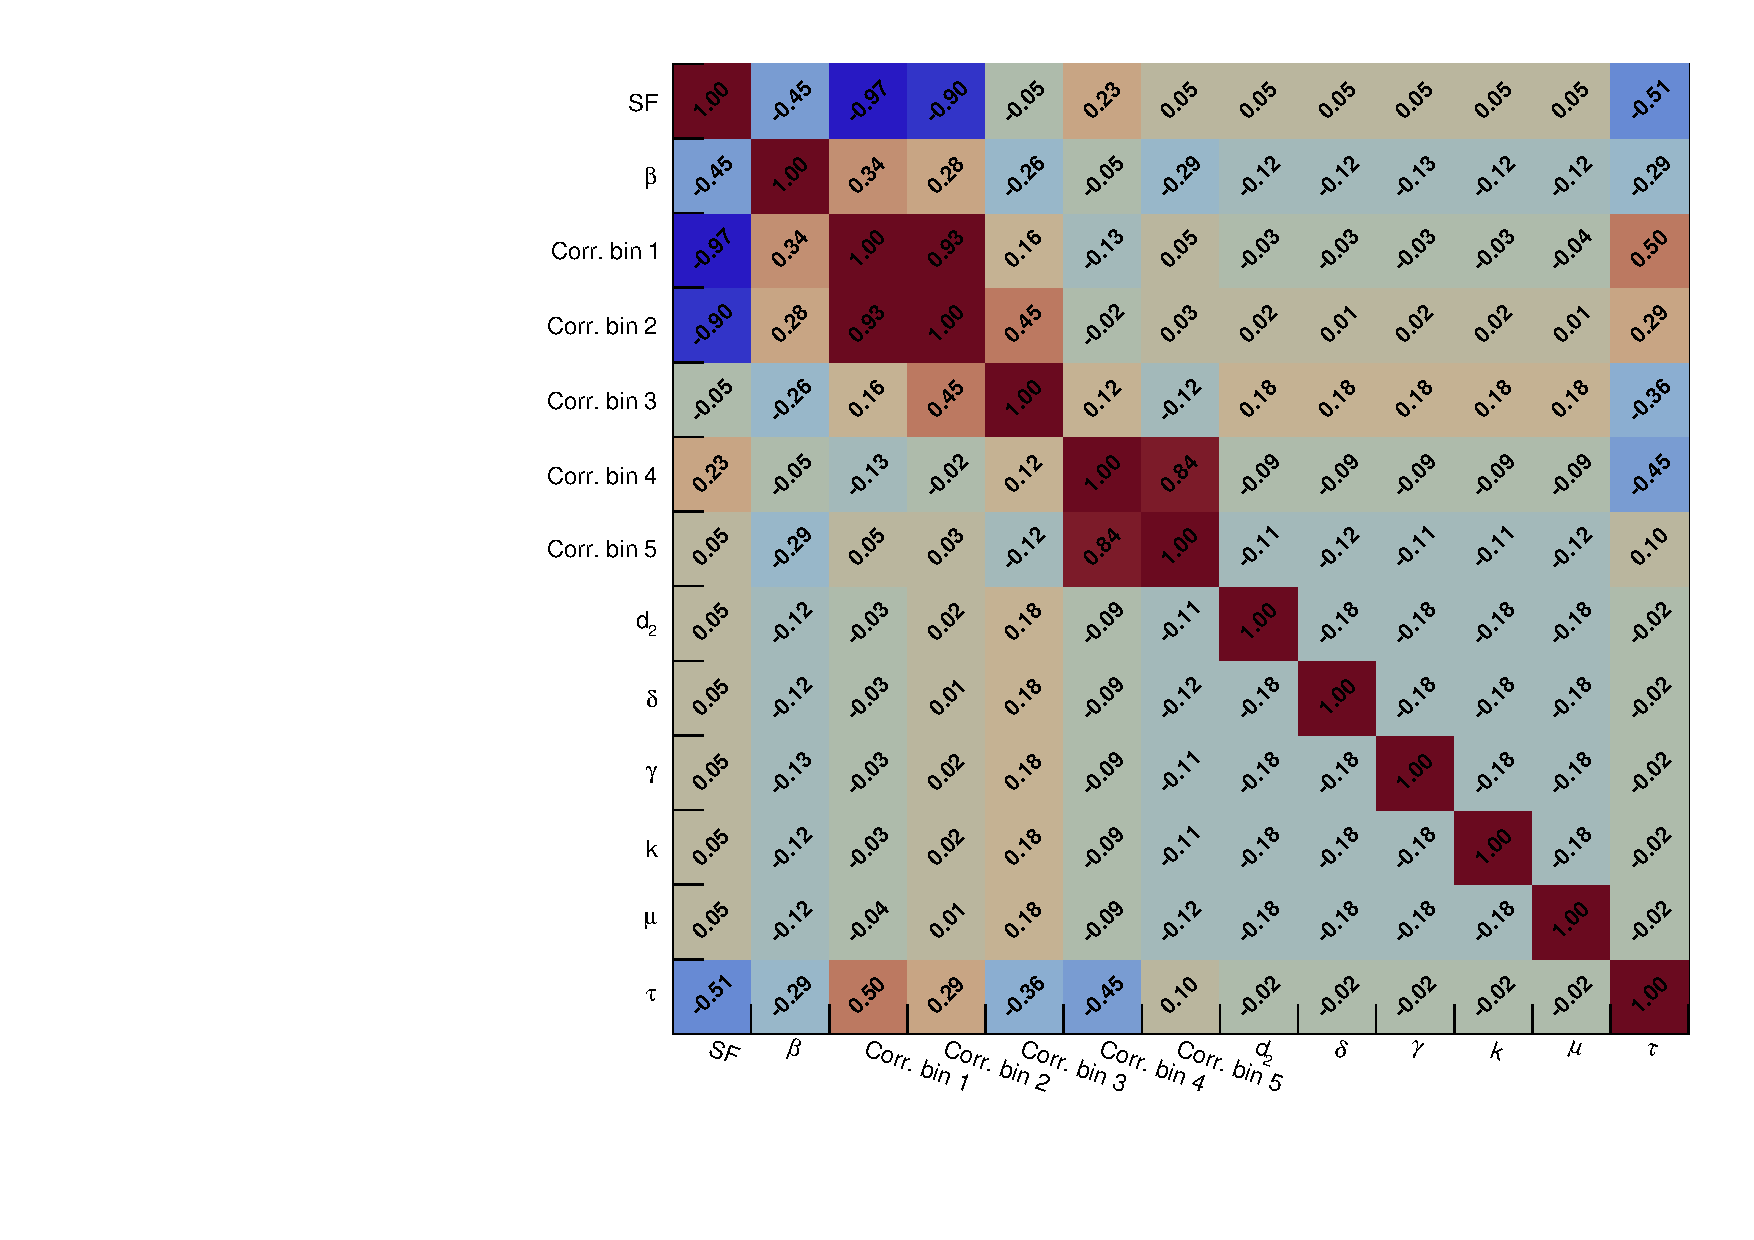
\includegraphics[width=0.4\textwidth]{imgs/Covid/CorrMatrix.pdf} }
  \caption{Fitted values of the model parameters (a). Correlations between the fitted parameters (b).}
  \label{fig:nps}
\end{figure}

The post-fit prediction is shown in Figure~\ref{fig:postfit}. The uncertainties are shrinked at higher bins, while enlarged in the lower bins because of the pulls and shows good agreement of the model with data within the fitted uncertainties.

\begin{figure}
\centering
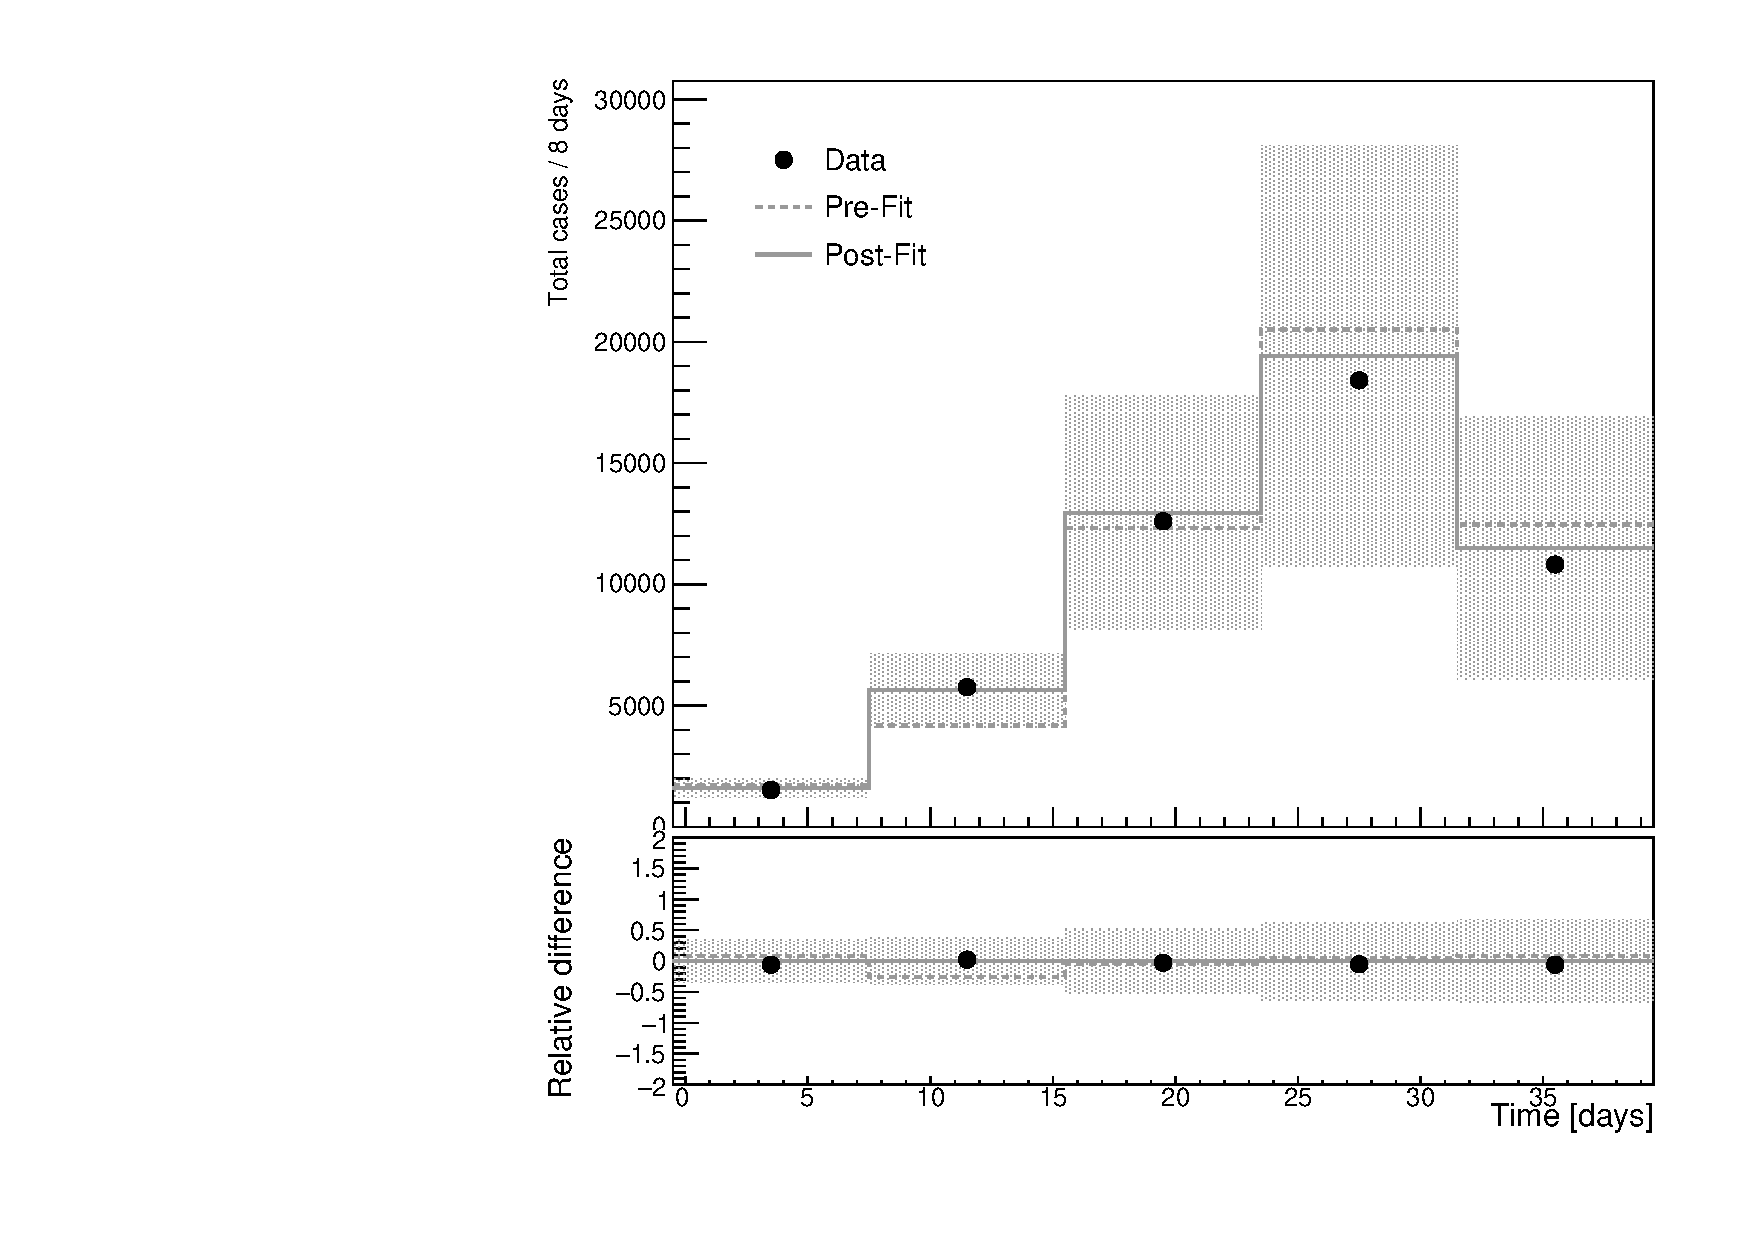
\includegraphics[width=0.4\textwidth]{imgs/Covid/ModelPostFit.pdf} 
  \caption{Post-fit prediction of the model with the corrections described in Figure~\ref{ssec:impr_model}, with parameters pulled as in Figure~\ref{fig:nps}a. The total uncertainty is given by summing all the post-fit uncertainties, correlated as in Figure~\ref{fig:nps}b.}
  \label{fig:postfit}
\end{figure}

\subsection{Predictions}
The fitted set of parameters is used to predict the evolution of the population categories evolutions, as shown in Figure~\ref{fig:model_postfit}a. In Figure~\ref{fig:model_postfit}b the evolution in time of $R_0$ is shown. $R_0$ stands for the infection power of each single individual. Here it is estimated as the ratio of the quarantined and infected (or just quarantined) population at time $t$ with the same quantity at time $t-\tau$, where $\tau $ is the incubation time. \\

\begin{figure}
\centering
\subfloat {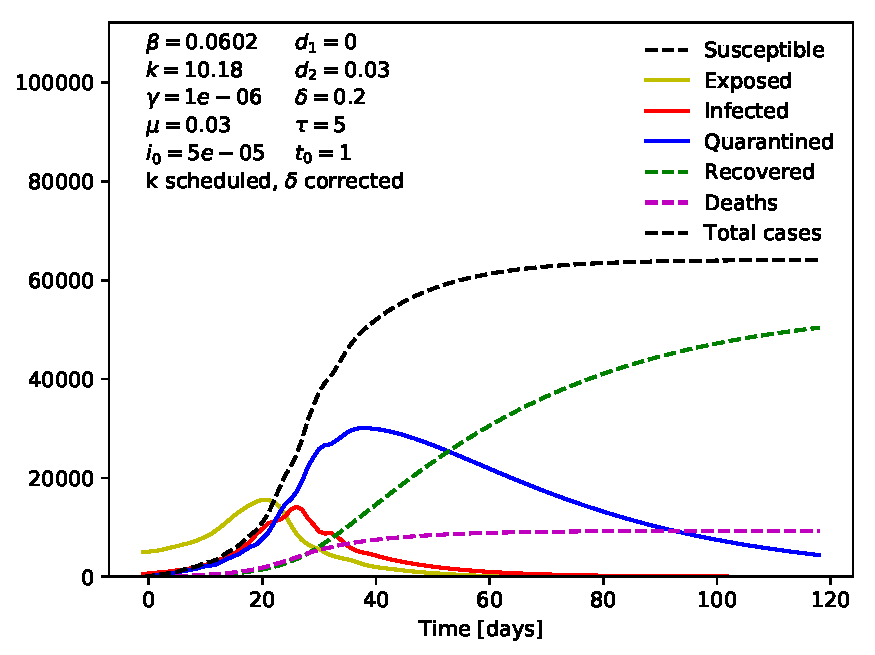
\includegraphics[width=0.4\textwidth]{imgs/Covid/Summary_parameters_Lombardia_scheduling_corrected_postfit_v2.pdf}  }
\subfloat {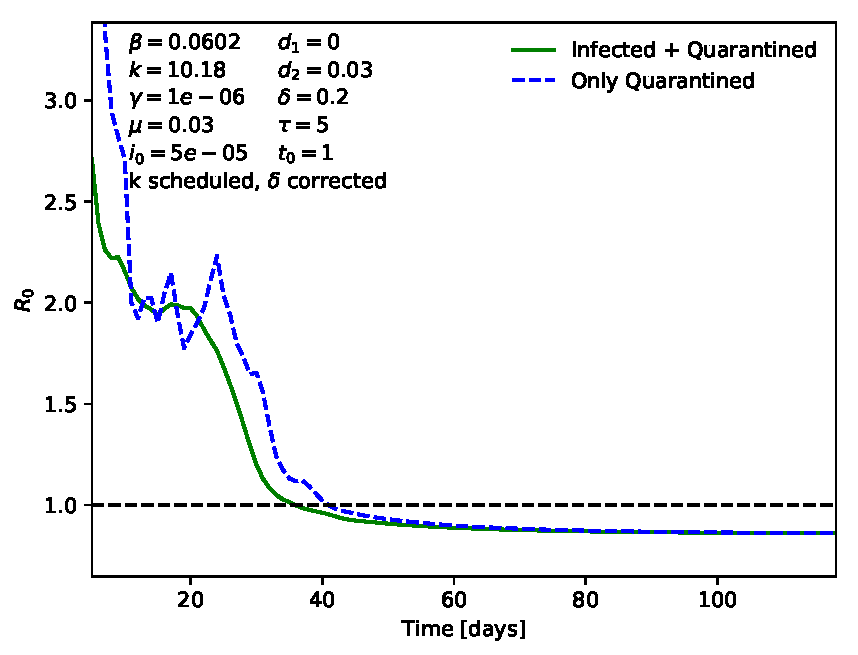
\includegraphics[width=0.4\textwidth]{imgs/Covid/R0_parameters_Lombardia_scheduling_corrected_postfit_v2.pdf}  }
  \caption{Prediction of the model tuned with the fitted parameters in Figure~\ref{fig:nps}a. Prediction of $R_0$ parameter against time (b).}
  \label{fig:model_postfit}
\end{figure}

The fitted model is used to predict some features of the virus spreading and to test them against the observations. To estimate the uncertainties on these estimations, a set of $1000$ pseudo-experiments is generated, obtained by extracting values of the model parameters from the fitted distributions, taking into account the fitted correlations. Predictions on a given observable are made by estimating mean and variance of the generated distribution from the pseudo-experiments. Since the fit is performed on the total cases distributions, predictions on the total cases related observables are more reliable. However, since quarantined population is the largest contribution to the total cases, especially in the fitted range, also the estimations of quarantined-related observables should be robust. The predictions on the number of deaths may be affected by the small contribution to the total cases in the fitted range, and therefore not very reliable. However, in the initial tuning (Figure~\ref{fig:model_vs_data}), the ratios between the contributions of the different classes is taken into account, so the obtained numbers should be in the same order of magnitude of the observations. A summary of the predictions on some observables of the outbreak evolution is given in Table~\ref{tab:predictions}.\\

\begin{table}\centering
\begin{tabular}{@{}lll@{}}
\toprule
Quantity & \phantom{abc} & Value \\
\midrule
\multicolumn{3}{@{}l@{}}{\emph{Quarantined people}}\\[1mm]
Peak & \phantom{abc} & $ 36000 \pm 21000 $\\
Peak time & \phantom{abc} & $ 38\pm1 $ days\\[3mm]

\multicolumn{3}{@{}l@{}}{\emph{Deaths}}\\[1mm]
Total deaths & \phantom{abc} & $ 13000 \pm 9000 $\\[3mm]

\multicolumn{3}{@{}l@{}}{\emph{Total cases}}\\[1mm]
Total & \phantom{abc} & $ 88000 \pm 67000 $\\
Saturation time & \phantom{abc} & $ 56\pm7 $ days\\
\bottomrule
\end{tabular}
\caption{Predictions of the model on some observables of the outbreak. The model is tuned with the fitted parameters in Figure~\ref{fig:nps}a. Dates are expressed in days after February 27th, the first day of available data.}
  \label{tab:predictions}
\end{table}

Currently (on 16/04/2020), from the updated data on reference \cite{Lab24}, there are $62153$ total cases, with $11377$ deaths. Both numbers are compatible with the predictions within the large uncertainties, but at least in the correct order of magnitude. The model predicts the peak of quarantined (positive) cases on April 2nd, however not a simple comparison with data is possible due to a lack of data documentation. The observed peak of daily new total cases is observed between March 21st and 26th, 2020: this is the highest slope of the total cases distribution against time, so expected earlier than the peak of quarantined population. A first decrease of total intensive in Italy care has been observed on April 4th, withing 2 standard deviations from the expectation. A comparison in terms of $R_0$ parameter is also possible.  The $R_0$ evolution, shown in Figure~\ref{fig:model_postfit}, can be tested as well. Considering the $R_0$ estimated only using quarantined population yields, an $R_0<1$ occurs around the 42th day, so on April 6th. The first indication of a $R_0<1$ in Italy is reported on April 9th \cite{R0}, quite close to the expectations. Unfortunately both  previous data are available only national-wise and not for Lombardy only, so results may differ. Finally, the estimated time of saturation of the total cases, corresponding to  reaching the $90\%$ of the maximum total cases, is expected in the week around April 20th.\\




\section{Conclusions}
The model looks to describe well the observation, even though the uncertainties are very large. However gives reliable indications on the shape of the oubreak and on the order of magnitude of the different classes of populations.


\begin{thebibliography}{9}
\bibitem{MingLiu} 
Z.~Gao, M.~Liu and Y.~Xiao, 
\textit{Modeling and Analysis of Epidemic Diffusion within Small-World Network},
Journal of Applied Mathematics (2012) 841531.

\bibitem{MingLiuOld} 
M.~Liu and L.~Zhao, 
\textit{Analysis for epidemic diffusion and emergency demand in an anti-bioterrorism
system},
International Journal of Mathematical Modelling and Numerical Optimisation (2011), vol. 2, no. 1, pp. 51–68.

\bibitem{COVID-Clinical} 
Jiang, F., Deng, L., Zhang, L. et al., \emph{ Review of the Clinical Characteristics of Coronavirus Disease 2019 (COVID-19)}, J GEN INTERN MED (2020).

\bibitem{Lab24}
Il Sole 24 Ore,
\textit{ 
Coronavirus in Italia, i dati e la mappa},
\href{https://lab24.ilsole24ore.com/coronavirus/}{https://lab24.ilsole24ore.com/coronavirus/}

\bibitem{WHO}
World Health Organisation, \emph{Coronavirus disease 2019 (COVID-19)}, \href{https://www.who.int/docs/default-source/coronaviruse/situation-reports/20200414-sitrep-85-covid-19.pdf?sfvrsn=7b8629bb_4}{Situation report, 85.}

\bibitem{DPCM-0903}
Presidenza del Consiglio, \emph{Decreto del presidente del consiglio dei ministri}, \href{http://www.trovanorme.salute.gov.it/norme/dettaglioAtto?id=73629}{Atto 73629, 09/04/2020}.

\bibitem{DPCM-1103}
Presidenza del Consiglio, \emph{Decreto del presidente del consiglio dei ministri}, \href{http://www.trovanorme.salute.gov.it/norme/dettaglioAtto?id=73643}{Atto 73643, 11/04/2020}.

\bibitem{DPCM-2003}
Presidenza del Consiglio, \emph{Decreto del presidente del consiglio dei ministri}, \href{http://www.trovanorme.salute.gov.it/norme/dettaglioAtto?id=73717}{Atto 73717, 20/04/2020}.

\bibitem{DPCM-2203}
Presidenza del Consiglio, \emph{Decreto del presidente del consiglio dei ministri}, \href{http://www.trovanorme.salute.gov.it/norme/dettaglioAtto?id=73728}{Atto 73728, 22/04/2020}.

\bibitem{DPCM-1004}
Presidenza del Consiglio, \emph{Decreto del presidente del consiglio dei ministri}, \href{https://www.gazzettaufficiale.it/atto/serie_generale/caricaDettaglioAtto/originario?atto.dataPubblicazioneGazzetta=2020-04-11&atto.codiceRedazionale=20A02179&elenco30giorni=true
}{, 10/04/2020}.

\bibitem{ROOT}
I.Antcheva et al., 
\textit{ 
ROOT — A C++ framework for petabyte data storage, statistical analysis and visualization},
Computer Physics Communications (2009), vol. 180, no. 12.

\bibitem{HistFactory}
Cranmer, Kyle and Lewis, George and Moneta, Lorenzo and Shibata, Akira and Verkerke, Wouter,
\textit{ 
HistFactory: A tool for creating statistical models for use with RooFit and RooStats},
CERN-OPEN-2012-016.

\bibitem{CaloTerapie}
Agenzia Nazionale Stampa Associata, 
\textit{Coronavirus: Calano malati in terapia intensiva, è la prima volta. In Lombardia in giro con le mascherine},
\href{https://www.ansa.it/canale_saluteebenessere/notizie/sanita/2020/04/04/coronavirus-_29e301b7-fd53-405c-9e5d-92f907057932.html}{Salute\&Benessere, 05 Aprile 2020.}

\bibitem{R0}
Ministero della Salute, \textit{Covid-19, Ministro Speranza: ``Vicini a R con zero inferiore a 1, ma la sfida non è vinta'' },
\href{http://www.salute.gov.it/portale/news/p3_2_1_1_1.jsp?lingua=italiano&menu=notizie&p=dalministero&id=4429}{News, 9 Aprile 2020.}

\end{thebibliography}


\newpage
\begin{appendices}
\section{Impact of parameters on model predictions}
Here the impact of the parameters on the model predictions is shown. The most important parameters for the evolution of the infected population and the occurrence of the outbreak are $\beta$ and $\braket{k}$ parameters. The $\beta$ parameters is connected to the infection factor, so the probability of infecting a susceptible person in contact with and infected one. The $\braket{k}$ parameters indicate instead the number of connection for each individual, so measures the level of interaction of the Small-World. Since the two parameters always come together their effect is the same on the evolution and visible in Figure~\ref{fig:scan_i_vs_beta}, the larger those parameters are the steeper the curve of the infected population is, as expected from Equation~\ref{eqn:idot}.  A large impact on the outbreak evolution is also given by the fraction of quarantined infected population $\delta$, as shown in Figures~\ref{fig:scan_i_vs_delta} and \ref{fig:scan_q_vs_delta}. The outbreak is significantly contained in case a larger fraction of infected population is spotted and quarantined.

\begin{figure}[!ht]\centering
\subfloat[\label{fig:scan_i_vs_beta}]{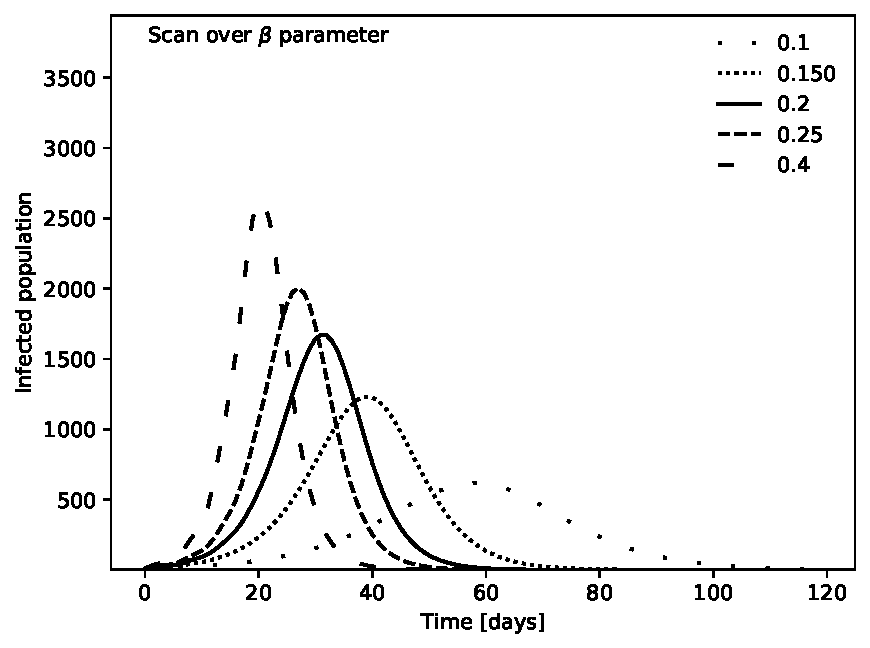
\includegraphics[width=0.32\textwidth]{imgs/ModelDescription/Scan_I_vs_beta_parameters_alternative.pdf}}
\subfloat[\label{fig:scan_i_vs_delta}]{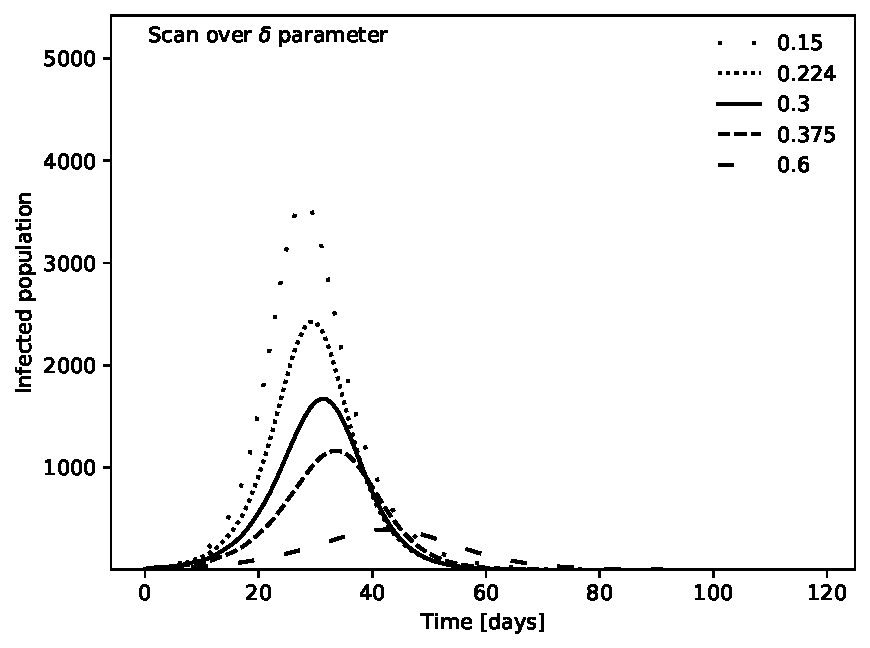
\includegraphics[width=0.32\textwidth]{imgs/ModelDescription/Scan_I_vs_delta_parameters_alternative.pdf}}
\subfloat[\label{fig:scan_q_vs_delta}]{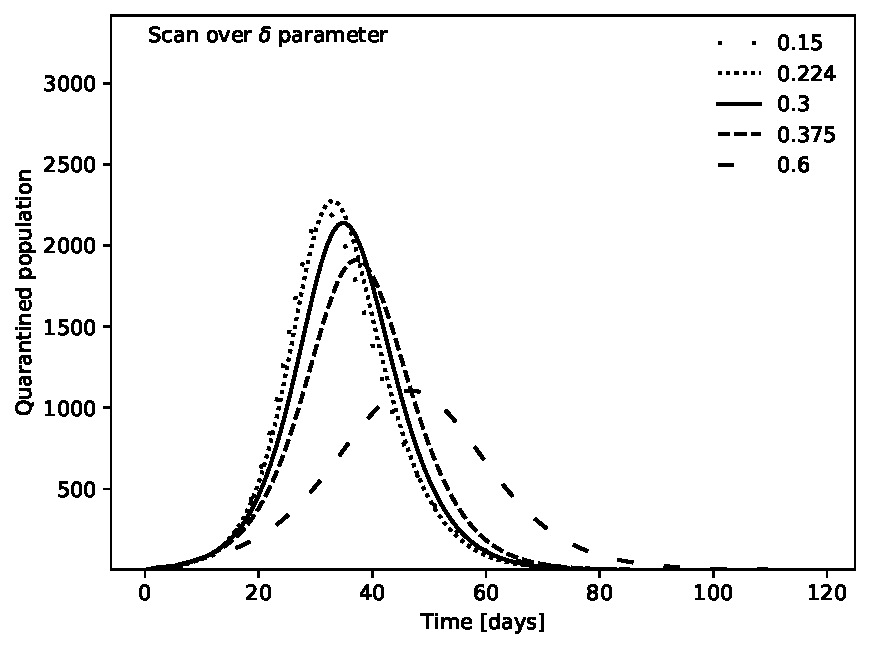
\includegraphics[width=0.32\textwidth]{imgs/ModelDescription/Scan_Q_vs_delta_parameters_alternative.pdf}}
\caption{Effect on the evolution of the infected population given by varying the $\beta$ parameter (a). Effect on infected (b) and quarantined (c) population given by varying the $\delta$ parameter.}.
\end{figure}

Other effects are given by $\gamma$, $\mu$ and $d_{1/2}$ parameters. Those control more the recovery curve. The $\gamma$ parameter is related to the probability of a recovered individual to not develop immunity: as shown in Figure~\ref{fig:scan_r_vs_gamma}, the recovered people has a decrease after the peak of the outbreak. The recovery curve is strongly affected by the $\mu$ parameter that regulates the recovery probability of the infected population, as shown in Figure~\ref{fig:scan_r_vs_mu}. The mortality $d_{1/2}$ instead increases the number of deaths, given by the difference of the recovered population and the initial $10000$ susceptible people, shown in Figure~\ref{fig:scan_r_vs_d1}.

\begin{figure}[!ht]\centering
\subfloat[\label{fig:scan_r_vs_gamma}]{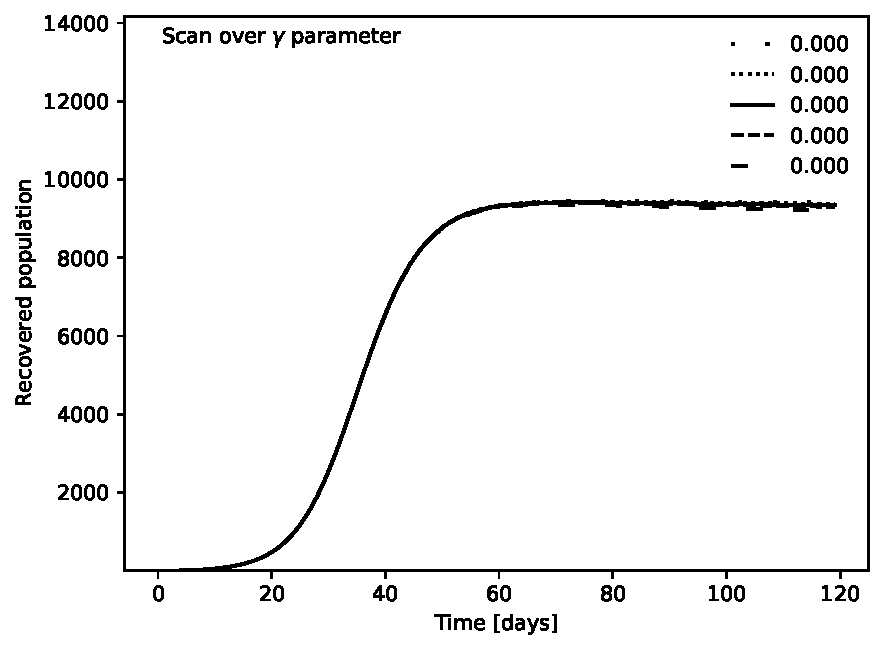
\includegraphics[width=0.32\textwidth]{imgs/ModelDescription/Scan_R_vs_gamma_parameters_alternative.pdf}}
\subfloat[\label{fig:scan_r_vs_mu}]{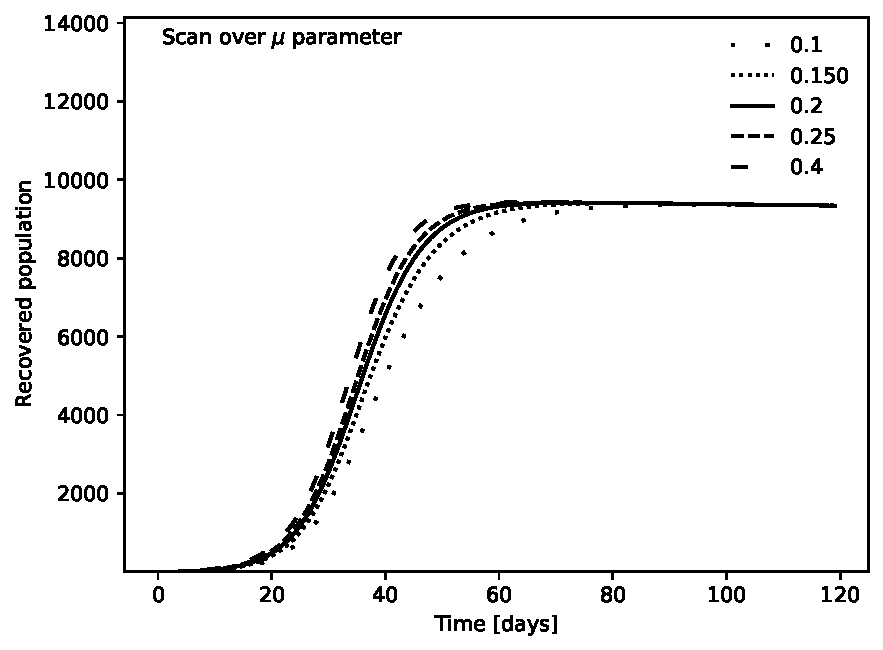
\includegraphics[width=0.32\textwidth]{imgs/ModelDescription/Scan_R_vs_mu_parameters_alternative.pdf}}
\subfloat[\label{fig:scan_r_vs_d1}]{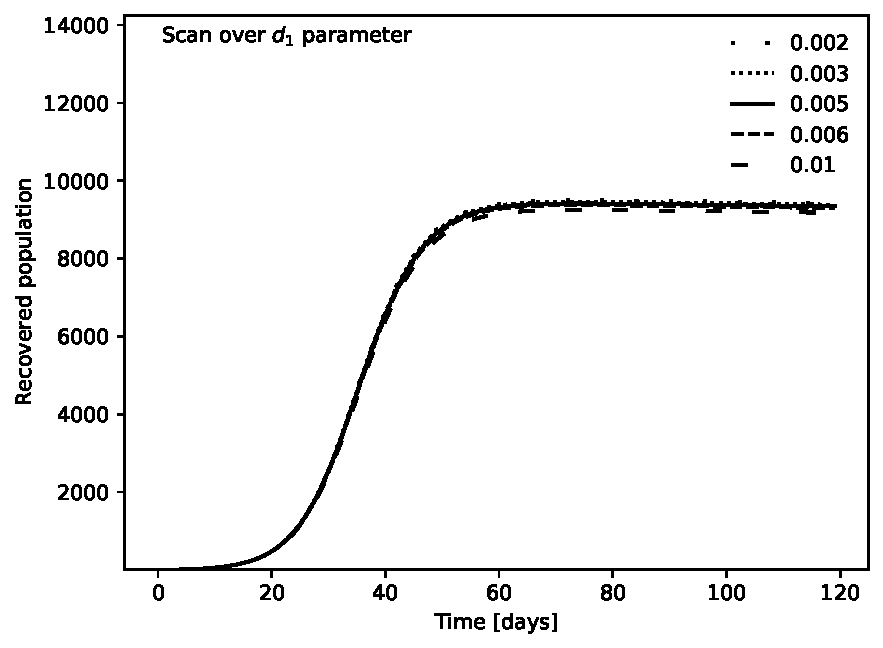
\includegraphics[width=0.32\textwidth]{imgs/ModelDescription/Scan_R_vs_d1_parameters_alternative.pdf}}
\caption{Effect on the evolution of the recovered population given by varying the $\gamma$ (a), $\mu$ (b) and $d_1$ (c) parameters.}.
\end{figure}

The only temporal parameter is the incubation time $\tau$: it also strongly affects the evolution of the oubreak, shown in Figure~\ref{fig:scan_i_vs_tau}. In case of long incubation time, the outbreak develops a  multiple peak structure, while in case of a short incubation time a clean ``gaussian'' peak is recognised.

\begin{figure}[!ht]\centering
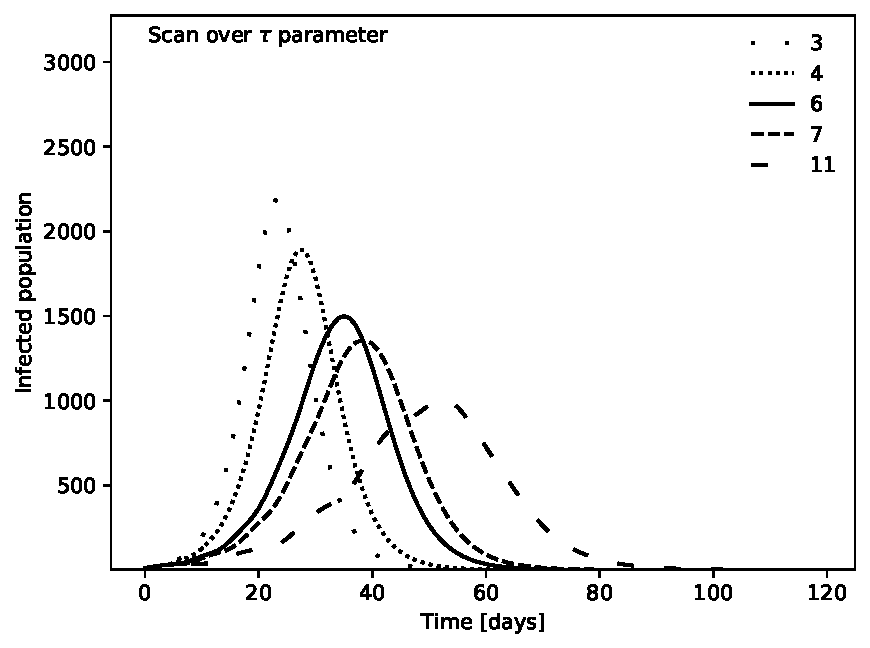
\includegraphics[width=0.4\textwidth]{imgs/ModelDescription/Scan_I_vs_tau_parameters_alternative.pdf}
\caption{Effect on the evolution of the infected population given by varying the $\tau$ parameter.}
\label{fig:scan_i_vs_tau}
\end{figure}

\end{appendices}

\end{document}
